% !TEX TS-program = pdflatex
% !TEX encoding = UTF-8 Unicode 
\documentclass[a4paper,11pt,openright,BCOR=15mm]{scrbook}

\usepackage[onehalfspacing]{setspace}    %   
\usepackage[utf8]{inputenc}
\usepackage[portuges,english]{babel}     
\usepackage[square,numbers]{natbib}
\usepackage{graphicx}               
\usepackage[pdftex]{hyperref}
\usepackage[T1]{fontenc}          
\usepackage{pdfpages}         
\usepackage{lettrine}    
\usepackage{booktabs}  
\usepackage{scrhack}   
\usepackage{scrlayer-scrpage}
\usepackage{ulem} % for underline
\usepackage{xcolor}
\definecolor{cinza1}{RGB}{200,200,200}
\definecolor{cinza2}{RGB}{70,70,70}
\usepackage{vhistory}	%% para versoes....
\newcommand\ChapterFont{}      % usar o tipo de letra normal
\newcommand\SectionFont{}
\pagestyle{scrheadings}
\ifoot[]{\raisebox{-32pt}{
\includegraphics[width=0.15\textwidth]{logos/logoisep}}}
\ofoot[]{\raisebox{-22pt}{
\includegraphics[width=0.10\textwidth]{logos/logo_DEI_big_transparente}}}
\cfoot[\pagemark]{\pagemark}
\automark[section]{chapter}
\usepackage{blindtext}   % \texto para demos 
\usepackage{listings}   %  para listagens com diferentes tipos de letra
\usepackage{fancyvrb}  %  para listagens de codigo 
\usepackage{float}

%%%%%%%%%%%%%%%%%%%%%%%%%%%%%%%%%%%%%%%%%%%%%%%%%%%%%%%%%%%%%%%%%%%%%%%%%%%%
\usepackage[mono=false]{libertine}
%%%%%%%%%%%%%%%%%%%%%%%%%%%%%%%%%%%%%%%%%%%%%%%%%%%%%%%%%%%%%%%%%%%%%%%%%%%%%%%%%%%%%%%%%

\begin{document}
	
	\selectlanguage{english}  
	\frontmatter
	
	\titlehead{
\includegraphics[scale=0.2]{figs/logoisep}
		\hfill 
\includegraphics[scale=0.115]{logos/logo_DEI_big_transparente}
	}  
	
	\title{Project (First Part) \\ \underline{Individual report} 
		}
	\subtitle{QSOFT}
	
	\author{Master in Informatics Engineering - 2024/2025}        
	
	
\publishers
{
	Pedro Miguel Santos Coelho\\    \texttt{Version \vhCurrentVersion, \vhCurrentDate}\\
}         
  
	
	
	
	\date{Porto, \today} 
	
	
	\maketitle   
	
	
	% Start of the revision history table
	\begin{versionhistory}
		\vhEntry{1}{2024-11-26}{Pedro Coelho}{Initial version}  
		\vhEntry{2}{2024-11-26}{Pedro Coelho}{Maintainability}
		\vhEntry{3}{2024-11-30}{Pedro Coelho}{Accessibility}
		\vhEntry{4}{2024-12-02}{Pedro Coelho}{Visual compatibility}
		\vhEntry{5}{2024-12-03}{Pedro Coelho}{Backend Performance}
		\vhEntry{6}{2024-12-05}{Pedro Coelho}{Backend Performance finish}
	\end{versionhistory}
	
	\cleardoublepage
	

	
	
	
	\tableofcontents
	\addcontentsline{toc}{chapter}{List of Figures}
	\listoffigures
	
	
	
	% \listoftables 
	
	\mainmatter 
	
	%% =================================
	

	%% =================================
	\chapter{Introduction}
	
\textit{This individual report focuses on the specific contributions made to the second phase of the QSOFT project. The primary objective was to analyze and improve a JHipster-generated monolithic application by addressing key quality attributes: accessibility, visual compatibility, maintainability, performance, and security. My tasks included checking the accessibility using LightHouse and generating a HTML report with the accessibility statment of the application, check the Visual compatibility of the application on different endpoints with different devices and sizes, check the maintainability of the current application and verify the performance of the backend and frontend of the application, ensuring compliance with the Goal-Question-Metric (GQM). The report details my individual approach, methodologies, and results, providing insights into how these tasks contributed to the overall project goals.}
	
		%% =================================
\chapter{Accessibility}

\textit{Web accessibility aims to develop digital content and applications that can be used by everyone, regardless of their physical, sensory, or cognitive abilities. This involves creating interfaces and features that are intuitive and functional for any user, promoting a barrier-free digital experience. The core idea is to ensure equal access to information and enable effective and inclusive interaction with the online environment.}
		
\section{LightHouse}
To assess the accessibility of a front-end application, I will use Lighthouse, a tool designed to analyze web applications and provide detailed feedback on accessibility issues. Lighthouse helps identify areas that need improvement, ensuring the application becomes more inclusive for all users.

In addition, ARIA (Accessible Rich Internet Applications) attributes will be applied when necessary. These attributes add semantic meaning to HTML elements, improving navigation and interaction for users who rely on assistive technologies such as screen readers. This process focuses on evaluating and enhancing the accessibility of the selected front-end page.

The page I evaluated was the visualise page for the petType. As shown in Figure \ref{fig:NivelAcessibilidade}, the application scored 96 out of 100 on the accessibility scale. This high score indicates that the front end developed for this page adheres to key principles of web accessibility, providing a positive and inclusive experience for users.


\begin{figure}[H]
	\centering
	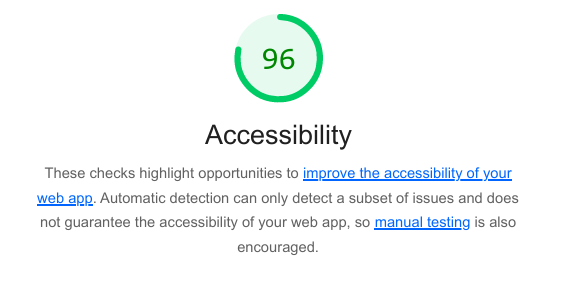
\includegraphics[width=\textwidth]{figs/Accessibility/NivelAcessibilidade.png}
	\caption{Accessibility Level before changes}
	\label{fig:NivelAcessibilidade}
\end{figure}

Following the report generated by the Lighthouse application, I identified that the main issue affecting accessibility is related to color contrast, as seen in the figure \ref{fig:NivelContraste}. 

Specifically, the contrast between foreground and background colors is insufficient, making it difficult or impossible for many users to read the text.

This issue is due to the application being generated with JHipster, which includes a red development banner by default. The low contrast between the banner's text and background contributes to the reported problem. To address this, adjustments to the color scheme will be required to ensure sufficient contrast and improve readability for all users.


\begin{figure}[H]
	\centering
	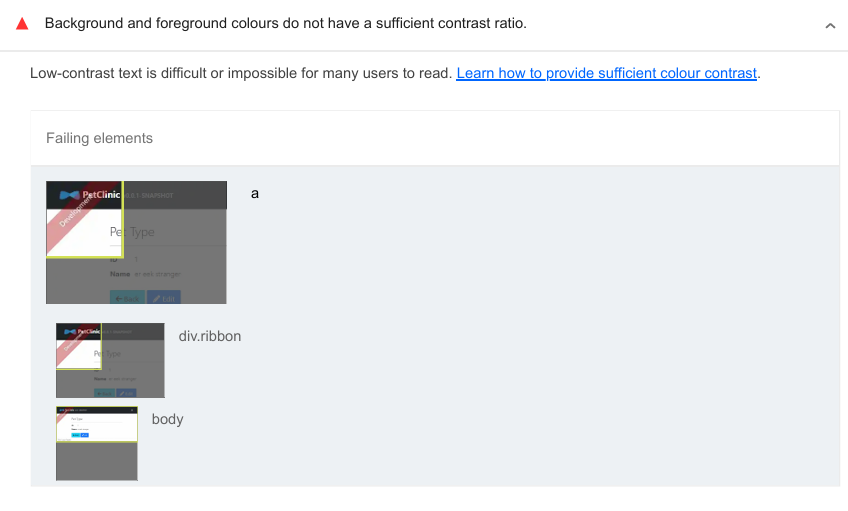
\includegraphics[width=\textwidth]{figs/Accessibility/NivelContraste.png}
	\caption{Contrast report}
	\label{fig:NivelContraste}
\end{figure}

If we were to remove the development banner added by default in JHipster, the Lighthouse accessibility score would reach 100\%, as this is the only issue identified in the report. The banner's insufficient color contrast is the sole factor affecting the accessibility evaluation, and its removal would ensure full compliance with accessibility standards, providing an optimal user experience.

\begin{figure}[H]
	\centering
	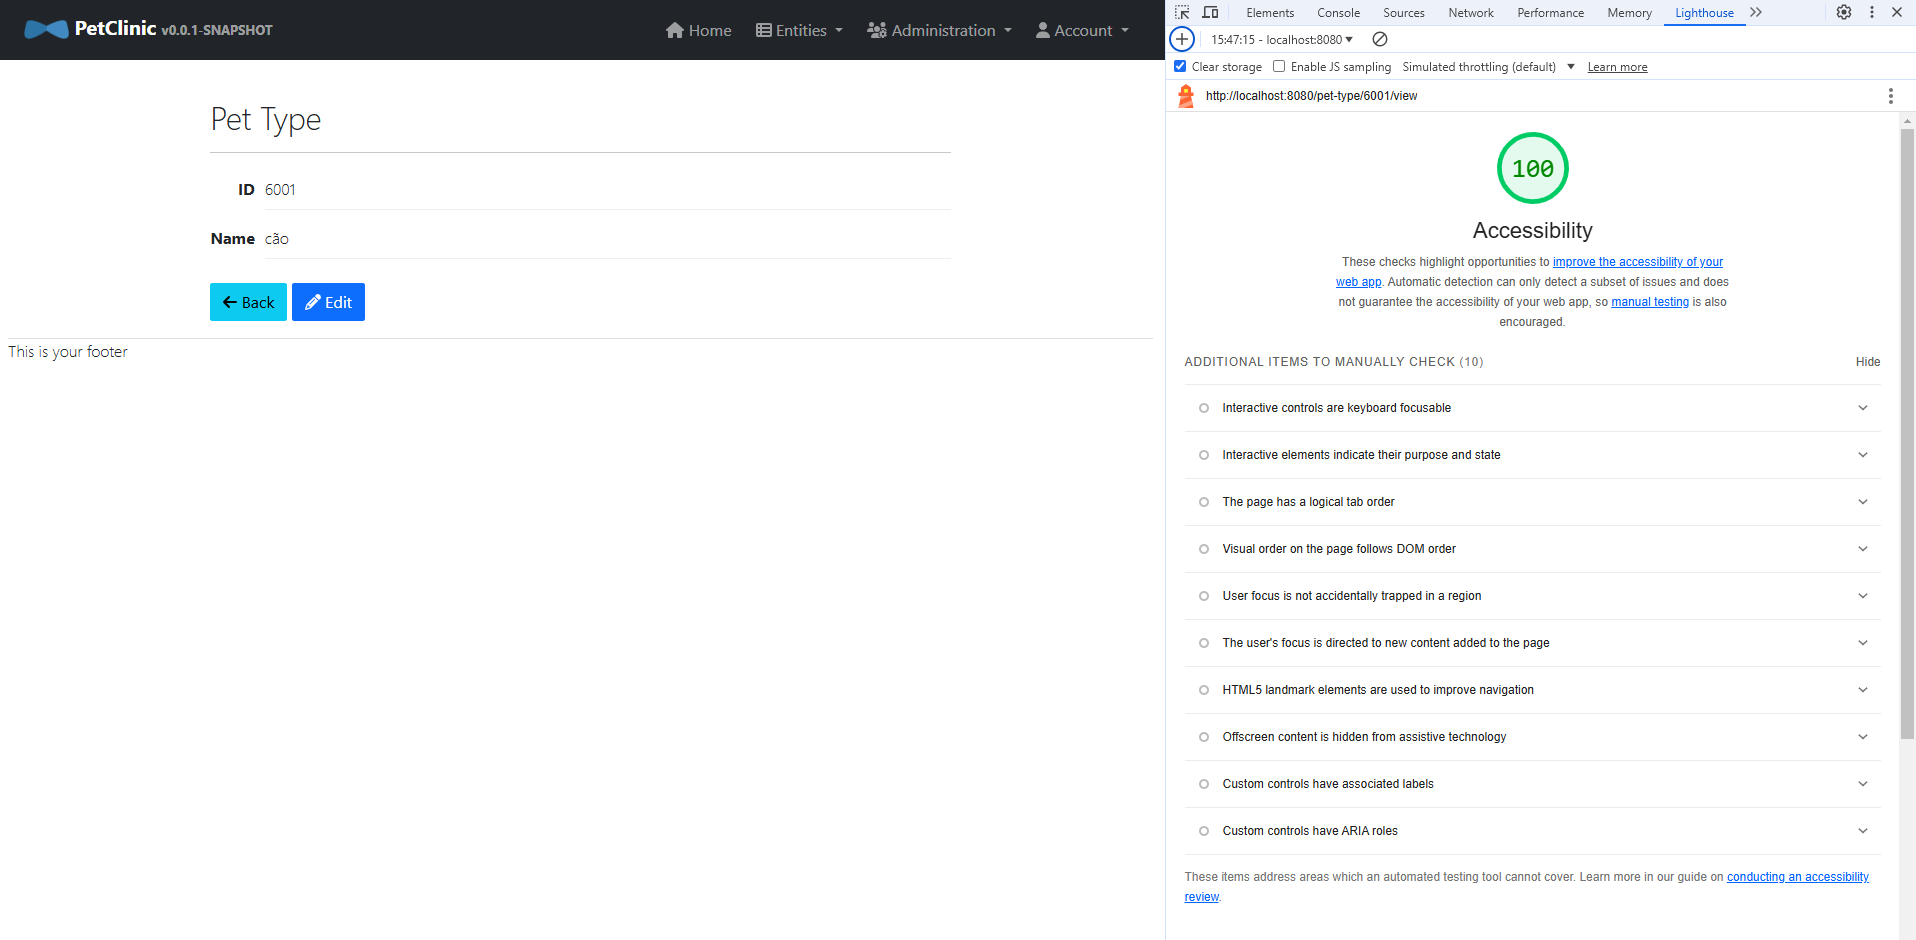
\includegraphics[width=\textwidth]{figs/Accessibility/NivelAcessibilidadeDepoisDaMudanca.png}
	\caption{Accessibility Level after changes}
	\label{fig:NivelContraste}
\end{figure}

In addition, I was able to navigate through the entire page using my keyboard, and the selected elements had an outline with a different color. However, in some areas, the color of the outline could be more noticeable as seen in the figure \ref{fig:BackSelected}.

\begin{figure}[H]
	\centering
	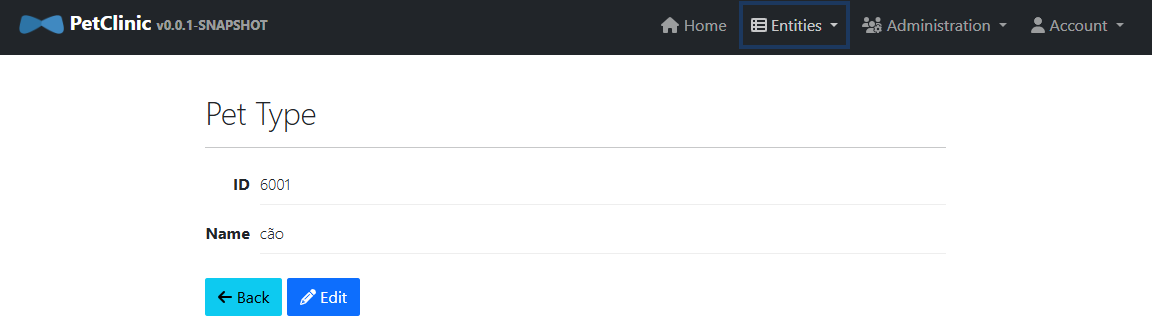
\includegraphics[width=\textwidth]{figs/Accessibility/Entities Selected.png}
	\caption{Navigate to Entities via Keyboard}
	\label{fig:EntitiesSelected}
\end{figure}

\begin{figure}[H]
	\centering
	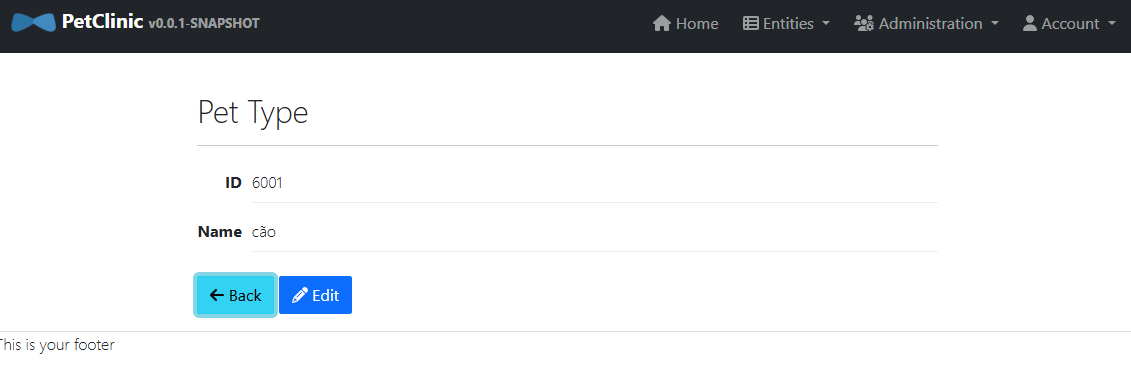
\includegraphics[width=\textwidth]{figs/Accessibility/Back Selected.png}
	\caption{Navigate to Back via Keyboard}
	\label{fig:BackSelected}
\end{figure}

\section{Web Accessibility Initiative}
By generating the Accessibility Statement from the \textit{https://www.w3.org} website, I ended up with the following HTML page. 

\begin{figure}[H]
	\centering
	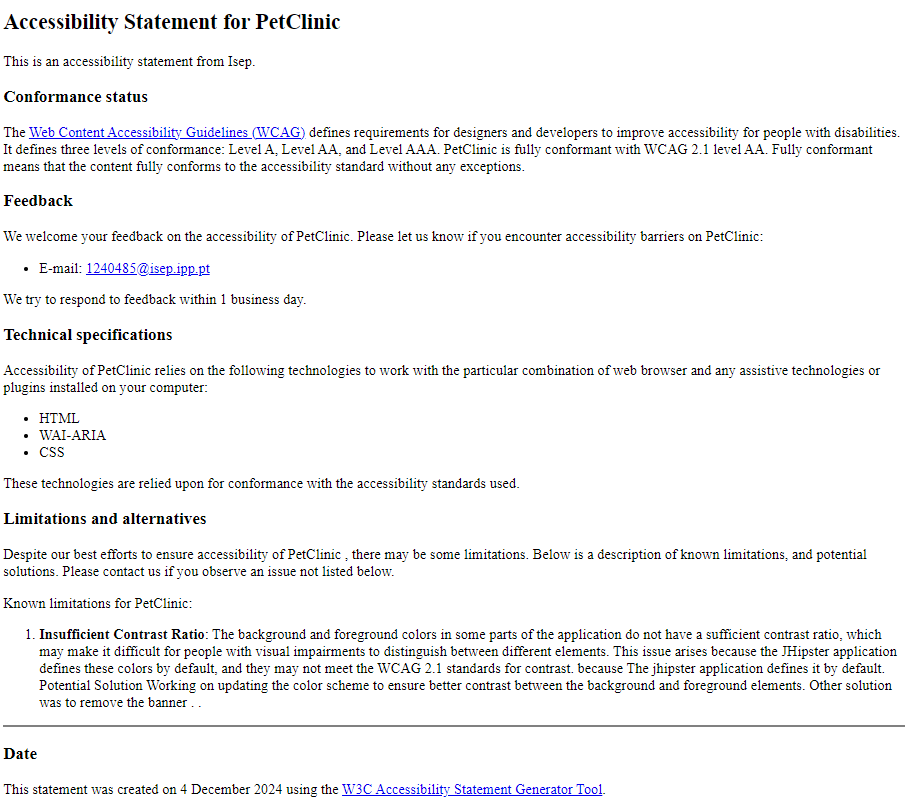
\includegraphics[width=\textwidth]{figs/Accessibility/HTML page.png}
	\caption{Html accessibility page}
	\label{fig:Html Page}
\end{figure}
Due to time constraints, I was unable to integrate this page into the project at the URL \textit{localhost:8080/pet-type/acessibilidade}. However, the HTML page can be found in the Accessibility folder of the 1240485 student.
\section{Conclusion}
The accessibility assessment of the application using Lighthouse revealed a strong performance, scoring 96 out of 100. The sole issue identified was related to the color contrast of the default "Development" banner generated by JHipster. Addressing this minor issue by either removing or adjusting the banner would result in a perfect accessibility score of 100\%, demonstrating the application's adherence to high accessibility standards.


Based on this, I rate the application of 5 out of 5 on accessibility chapter.
\chapter{Visual compatibility}
\textit{Visual compatibility refers to the seamless interaction of visual elements, ensuring they work harmoniously to create a cohesive and appealing design. It functions by balancing key factors such as color harmony, typography, proportion, layout, and style consistency. When these elements are thoughtfully integrated, they enhance the clarity, usability, and emotional resonance of a design.}
\section{Tests}
In the same way that we discussed accessibility in the previous chapter, I will now address the visual compatibility of the Visualise Page of PetTypes, in addition I will also analyze the List Page of the PetTypes.
The tests will be conducted with BackstopJS with the intention of verifying if the visualise page of the PetTypes Domain of our web application is readable across different devices, such as mobile phones and tablets or a computer.



\section{Scenarios}
In the figure \ref{fig:Scenarios} we can see the configuration for endpoints that are being tested in this chapter.


\begin{figure}[H]
	\centering
	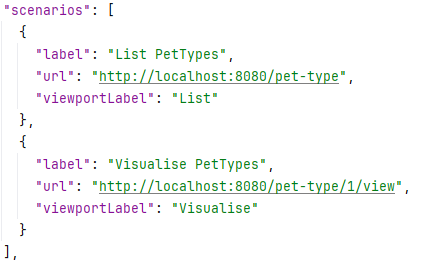
\includegraphics[width=.7\textwidth]{figs/Visual compatibility/Scenarios.png}
	\caption{Configuration on json for the endpoints}
	\label{fig:Scenarios}
\end{figure}
Considering that the application has an authentication system, the login was defined in the onBefore file to make the pages accessible during testing. This can be seen and verified in the figure \ref{fig:onBefore}
\begin{figure}[H]
	\centering
	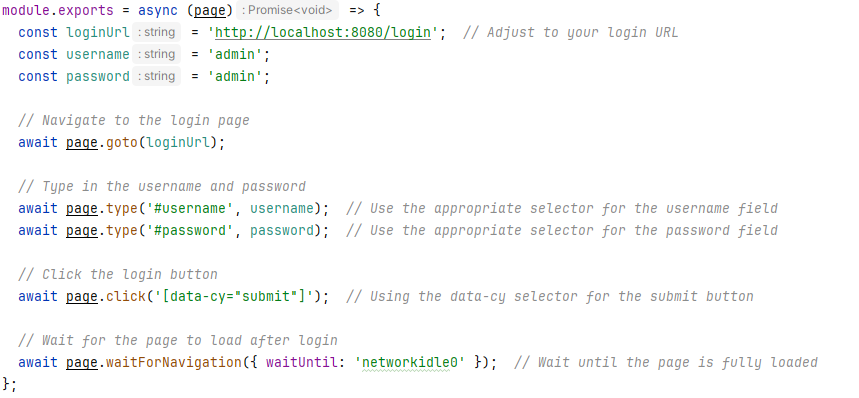
\includegraphics[width=.7\textwidth]{figs/Visual compatibility/onBefore.png}
	\caption{Configuration on onBefore.js for authentication}
	\label{fig:onBefore}
\end{figure}


\section{Viewports}
\subsection{Mobile Phones}
In the table below, we can see the dimensions used for the mobile phone tests. Below, in the figure \ref{fig:Mobile Phones}, we can observe the configuration file for mobile phone testing.

\begin{longtable}{|l|l|c|c|}
\hline
\textbf{Type} & \textbf{Label} & \textbf{Width (px)} & \textbf{Height (px)} \\
\hline
\endfirsthead
\hline
\textbf{Type} & \textbf{Label} & \textbf{Width (px)} & \textbf{Height (px)} \\
\hline
\endhead
Small Phone & small-phone & 320 & 480 \\
Medium Phone & medium-phone & 375 & 667 \\
Large Phone & large-phone & 414 & 896 \\
\hline
\end{longtable}

\begin{figure}[H]
	\centering
	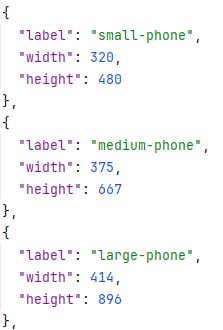
\includegraphics[width=.3\textwidth]{figs/Visual compatibility/Phone.png}
	\caption{Configuration on json for Mobile Phones}
	\label{fig:Mobile Phones}
\end{figure}

\subsection{Tablets}
n this section, we present the dimensions used for the tablet tests. Below, in the figure \ref{fig:Tablets}, we can observe the configuration file for tablet testing.
\begin{longtable}{|l|l|c|c|}
\hline
\textbf{Type} & \textbf{Label} & \textbf{Width (px)} & \textbf{Height (px)} \\
\hline
\endfirsthead
\hline
\textbf{Type} & \textbf{Label} & \textbf{Width (px)} & \textbf{Height (px)} \\
\hline
\endhead
Small Tablet & small-tablet & 768 & 1024 \\
Medium Tablet & medium-tablet & 1024 & 768 \\
Large Tablet & large-tablet & 1366 & 1024 \\
\hline
\end{longtable}

\begin{figure}[H]
	\centering
	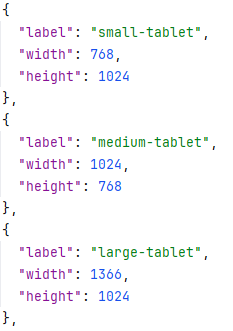
\includegraphics[width=.3\textwidth]{figs/Visual compatibility/Tablet.png}
	\caption{Configuration on json for Tablets}
	\label{fig:Tablets}
\end{figure}

\subsection{Desktops}
The table below shows the dimensions used for desktop tests. Below, in the figure \ref{fig:Desktop}, we can observe the configuration file for desktop testing.


\begin{longtable}{|l|l|c|c|}
\hline
\textbf{Type} & \textbf{Label} & \textbf{Width (px)} & \textbf{Height (px)} \\
\hline
\endfirsthead
\hline
\textbf{Type} & \textbf{Label} & \textbf{Width (px)} & \textbf{Height (px)} \\
\hline
\endhead
Small Desktop & small-desktop & 1024 & 768 \\
Medium Desktop & medium-desktop & 1280 & 1024 \\
Large Desktop & large-desktop & 1920 & 1080 \\
\hline
\end{longtable}

\begin{figure}[H]
	\centering
	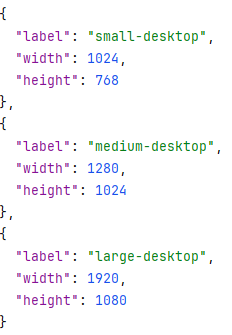
\includegraphics[width=.3\textwidth]{figs/Visual compatibility/Desktop.png}
	\caption{Configuration on json for Desktop}
	\label{fig:Desktop}
\end{figure}

\section{Test results}
In total, 18 tests were performed. These tests covered each endpoint (Visualise and List), across different device types (phone, tablet, desktop), and for various screen sizes (small, medium, large). As we can see in the figure \ref{fig:BackstopJS} all 18 tests passed, which means that the test images that came from the "backstop test" were exactly equal to the references images created from the "backstop reference". An example of this comparison can be seen in the figure \ref{fig:ResultExample}
\begin{figure}[H]
	\centering
	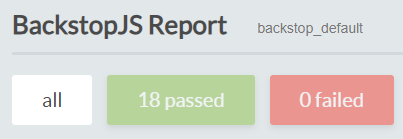
\includegraphics[width=.3\textwidth]{figs/Visual compatibility/BackstopJSReportResults.png}
	\caption{BackstopJS Results}
	\label{fig:BackstopJS}
\end{figure}
\begin{figure}[H]
	\centering
	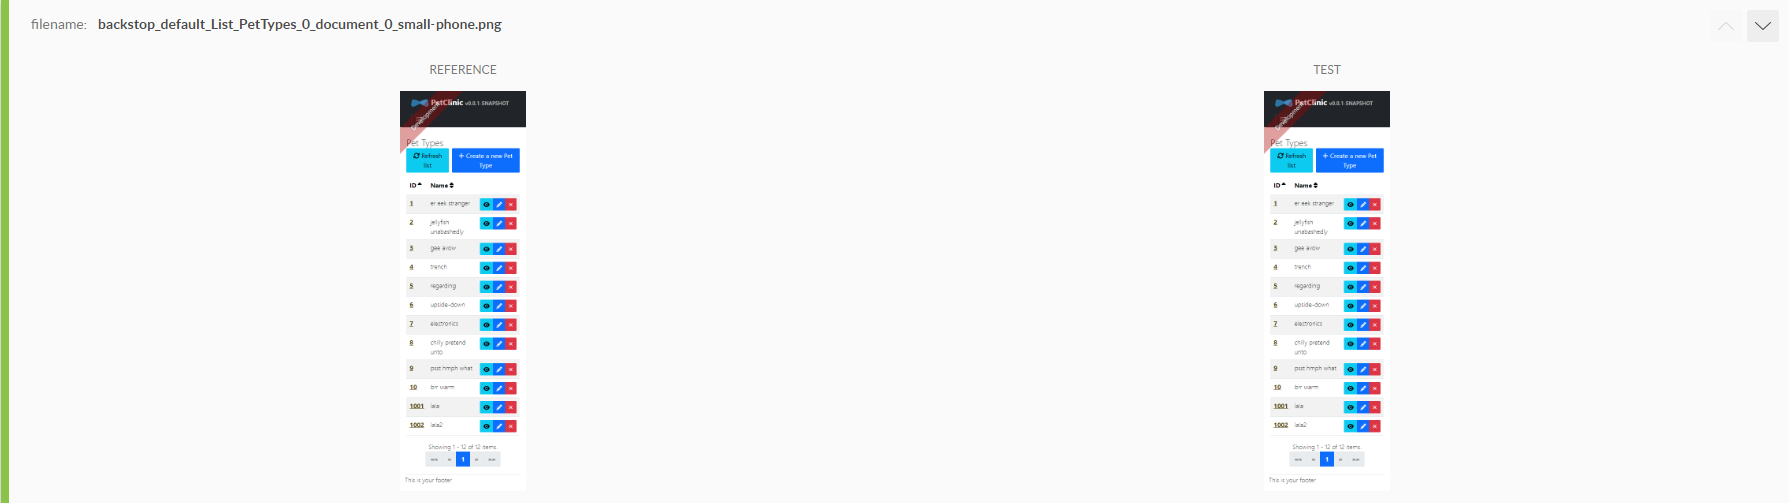
\includegraphics[width=\textwidth]{figs/Visual compatibility/ResultExample.png}
	\caption{BackstopJS Result Example}
	\label{fig:ResultExample}
\end{figure}


\section{Conclusion}
The visual compatibility tests conducted in this chapter provide a comprehensive assessment of the application’s interface consistency across various devices and screen sizes. Considering that all tests were successful, we can confirm that the application delivers a consistent and reliable visual experience, regardless of the device or screen size. This consistency is essential for maintaining a high-quality user experience across different platforms.


Based on these results, we can confidently conclude that the application meets the necessary standards for visual compatibility, and the overall performance in this area is rated 5 out of 5, reflecting flawless performance across all tested environments.


%% =================================	
\chapter{Maintainability}
\textit{	Maintainability refers to the ease with which a software system can be modified to adapt to new requirements, correct defects, or improve performance after deployment. It ensures the long-term sustainability and adaptability of the application. In this phase of the project, relevant maintainability metrics, such as Coupling, Structural Erosion, Size, and Complexity, will be analyzed. The assessment will be conducted using tools and methodologies aligned with best practices, as detailed in the following sections.}
\section{Coupling and Structural Erosion}
\begin{itemize}
    \item \textbf{Metric:} Average Component Dependency (ACD)
    \item \textbf{Category:} Cohesion/Coupling (John Lakos)
    \item \textbf{Value:} 4.36
\end{itemize}
As seen in the Figure \ref{fig:ACD} ACD value of 4.36 indicates that, on average, each component in the system depends on approximately 4 other components, both directly and indirectly. This relatively low level of dependency suggests a good degree of modularity within the architecture, where components are less tightly coupled. Such an architecture facilitates independent functionality and makes it easier to modify or refactor components with minimal risk of unintended interactions.

A lower ACD value generally reflects better maintainability, as the reduced dependencies increase the flexibility of individual components and decrease the likelihood of cascading changes when updates are made. This level of cohesion promotes a system design that is easier to evolve and maintain over time. However, it remains essential to ensure that the reduced dependency does not compromise the necessary interactions and integrations within the system.
\begin{figure}[H]
	\centering
	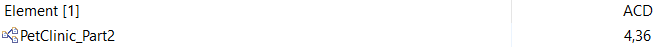
\includegraphics[width=\textwidth]{figs/Maintainability/ACD.png}
	\caption{ACD}
	\label{fig:ACD}
\end{figure}

\section{Size and Complexity}
\begin{itemize}
    \item \textbf{Metric:} Number of Components/Sources
    \item \textbf{Category:} Size
    \item \textbf{Value:} 107
\end{itemize}
As seen in the figure \ref{fig:NumberOfComponentsSources} project consists of 107 components or source files, which provides a structural overview of its size and organization. In the context of a codebase with approximately 5000 lines of code, the distribution of 107 components suggests an average of approximately 47 lines per component. This number indicates a relatively well-organized project structure, where code is compartmentalized across manageable components. Such organization enhances readability, traceability, and modularity, contributing to the maintainability of the system by making individual components easier to understand, modify, and test.
\begin{figure}[H]
	\centering
	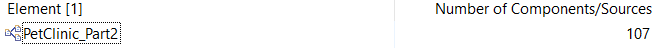
\includegraphics[width=\textwidth]{figs/Maintainability/Number of ComponentsSources.png}
	\caption{Number Of Components/Sources}
	\label{fig:NumberOfComponentsSources}
\end{figure}

\section{Conclusion}

The maintainability analysis of the project demonstrates strong adaptability and long-term sustainability. The Average Component Dependency (ACD) value of \textbf{4.36} reflects a modular architecture with low coupling, making the system easier to modify and reducing the risk of unintended interactions. Additionally, with \textbf{107 components} and an average of \textbf{47 lines of code per component}, the codebase is well-organized and modular, enhancing readability and ease of testing. These characteristics ensure the system's ability to evolve, address defects, and maintain performance over time.


Overall, the maintainability of the project is strong, with a well-organized, modular architecture and low coupling, ensuring long-term sustainability. However, there is still room for optimization, particularly in reducing dependencies and refining the number of components. Combining these factors, maintainability is rated 4 out of 5, reflecting a solid foundation with opportunities for further improvement.%% =================================		
	\chapter{Performance}
\textit{    Just like in the Project 1, I will be evaluating the performance of the application. However, unlike the first project, now I will evaluate the front-end performance of the application as well. In order to test the backend I will adapt the tests used in the project 1, both for the jmeter and for k6. To evaluate the performance of the frontend I used LightHouse, the same application used for the Accessibility chapter.     }		

\section{Testing Environment}
  All tests conducted for this evaluation were performed on a single machine/computer, with the specifications outlined in the image below (\ref{fig:SystemDetails}). It's important to note that the computer remained consistently connected to the internet via an Ethernet cable throughout the testing process. This ensures a consistent and standardized testing environment, allowing for accurate and reliable performance assessments under the specified configurations. The use of a wired connection guarantees stable network conditions, contributing to the precision of the results obtained during the evaluation.
  
  	\begin{figure}[h]
    	\centering
    	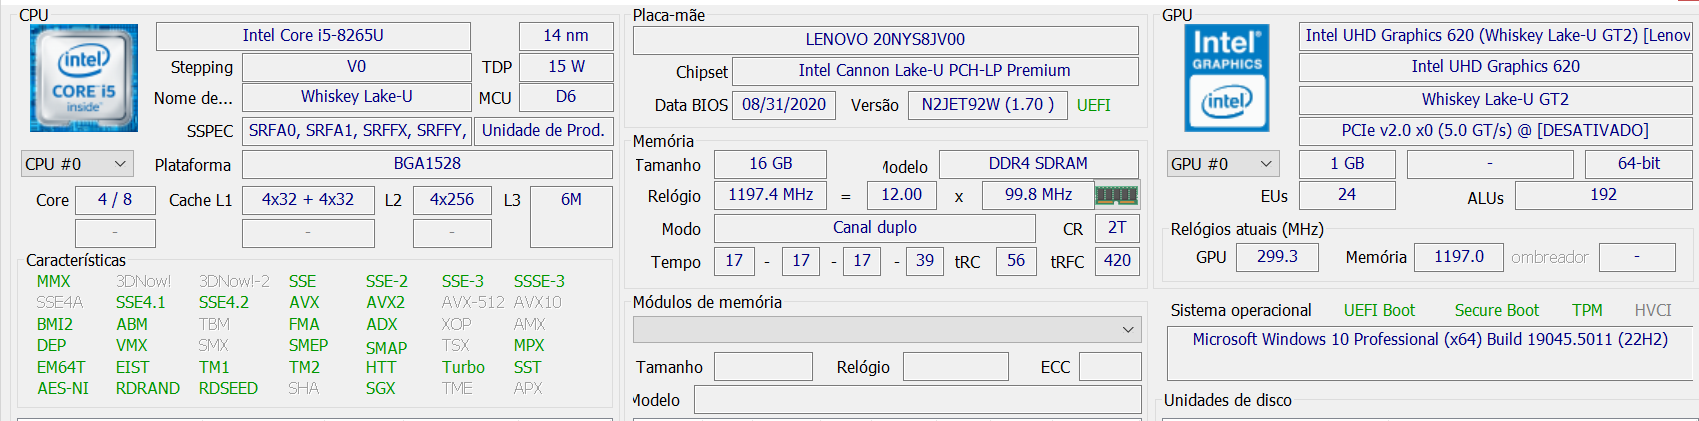
\includegraphics[width=\textwidth]{figs/Performance/SystemDetails.png}
    	\caption{System Details}
    	\label{fig:SystemDetails}
  	\end{figure}



\section{Backend performance}
In the following sections, we will explore specific performance metrics, analyze the
results obtained from JMeter and K6 tests, and draw conclusions about the project’s
suitability for integration into a larger system based on its performance attributes.

\subsection{Requirements}
\textbf{Normal Conditions}
\begin{itemize}
	\item Supports normal user access of 50 users.
	\item Respond to any type of request in less than 3 seconds 99\% of the time.
	\item Process more than 250 requests per second.
\end{itemize}



\textbf{Heavy Conditions}
\begin{itemize}
	\item Supports heavy user access of up to 200 users.
	\item Respond to any type of request in less than 5 seconds 99\% of the time.
	\item Process more than 150 requests per second.
\end{itemize}

\subsection{Authentication}
Due to the application requiring authentication to perform actions on its endpoints, it became necessary to generate a Bearer Token for use in JMeter and K6 tests. To accomplish this, I used Postman, as shown in the figure \ref{fig:Authentication}. By logging in with valid credentials, the application returns a token, which can then be used to authenticate subsequent requests in JMeter or K6 tests, as demonstrated later in the figure \ref{fig:Authenticationjmeter} for jmeter and in the figure \ref{fig:Authenticationk6}. This procedure is applied in all the tests presented in this chapter..
\begin{figure}[H]
	\centering
	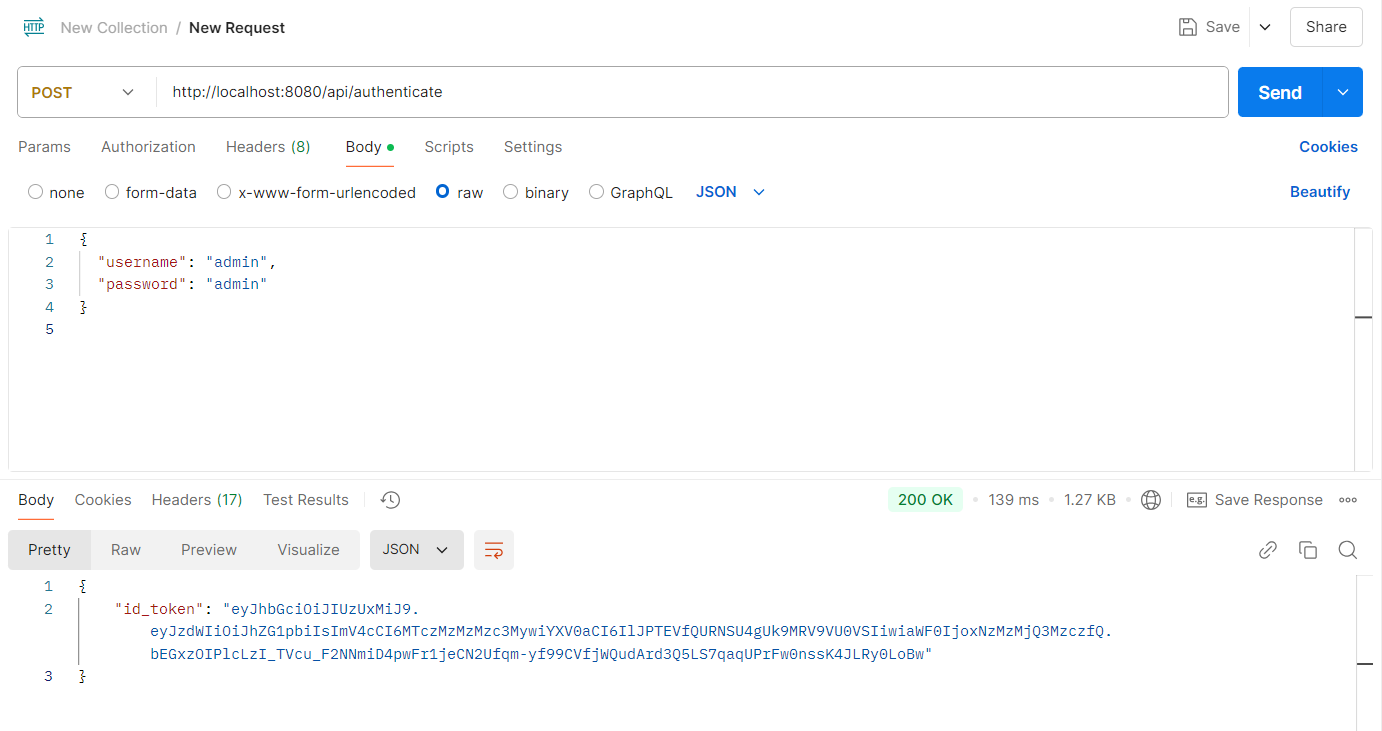
\includegraphics[width=\textwidth]{figs/Performance/Authentication.png}
	\caption{Authentication via Postman}
	\label{fig:Authentication}
\end{figure}
\begin{figure}[H]
	\centering
	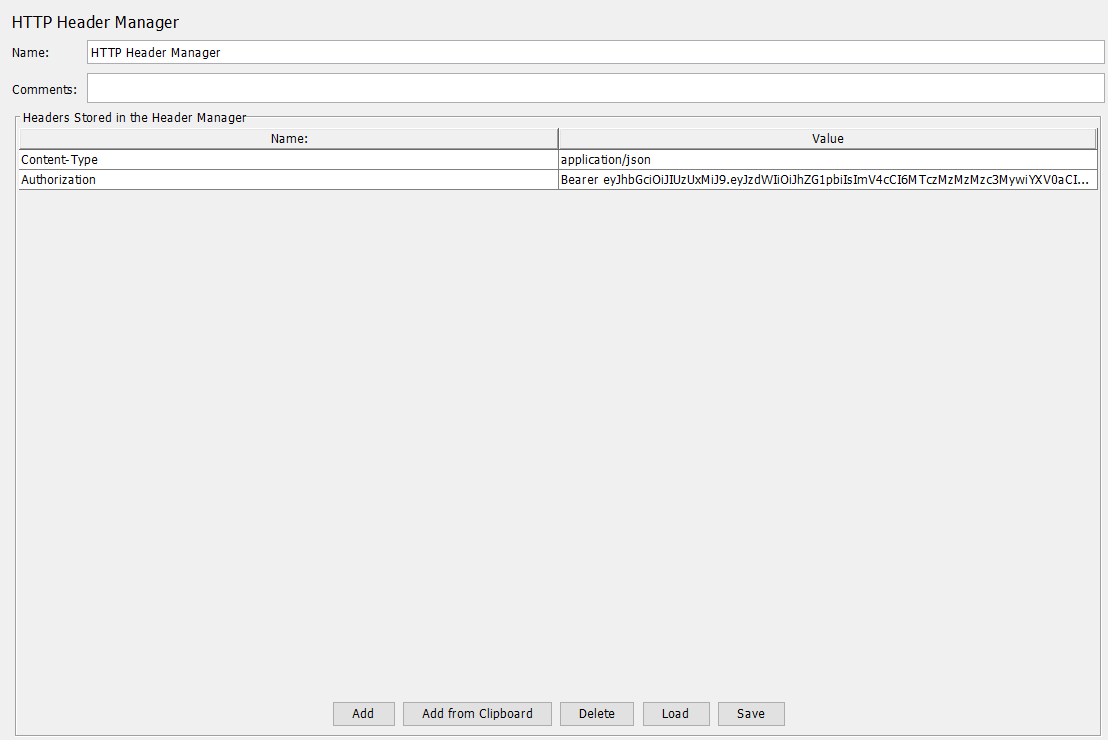
\includegraphics[width=\textwidth]{figs/Performance/AuthenticationjMeter.png}
	\caption{Usage of Token on jmeter tests}
	\label{fig:Authenticationjmeter}
\end{figure}
\begin{figure}[H]
	\centering
	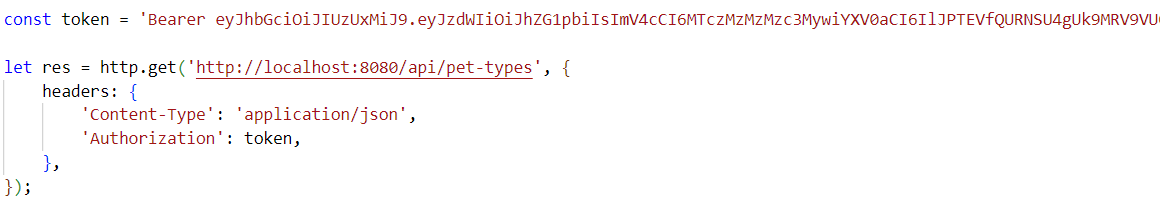
\includegraphics[width=\textwidth]{figs/Performance/Authenticationk6.png}
	\caption{Usage of Token on k6 tests}
	\label{fig:Authenticationk6}
\end{figure}

\subsection{Load Test}

Load testing evaluates a system's behavior under typical conditions by simulating realistic user activity. This process enables the early identification of performance issues, such as response time delays and resource overuse, even at normal load levels. Additionally, it provides insights into the system’s capacity, supporting scalability planning to ensure it can handle anticipated user growth effectively.
In this section we will evaluate the Loads tests to the endpoints POST of petType

\textbf{Scenario POST}

\begin{itemize}
	\item 50 users of the web application
	\item Posting a new PetTypes
	\item The system returns 201
	\item Normal Conditions
\end{itemize}

\textbf{Jmeter}




\textbf{Test Configuration}



In the figure \ref{fig:LoadCSVjmeter} we can see the configuration needed to load the csv file on jmeter, later, on the figure \ref{fig:LoadCSV2jmeter} we can see how to use the same data from the csv for the POST requests. In the figure \ref{fig:LoadConfigurationjMeter} we can see the configuration on jmeter for the test where we
can see that this test simulates a ramp-up to 50 virtual users over 10 seconds, maintains
this load for 90 seconds, and then ramps down to 0 users over 10 seconds. In the figure \ref{fig:LoadDurationjMeter} we can see the configuration for the duration for each request in jmeter of 3 seconds.

\begin{figure}[H]
	\centering
	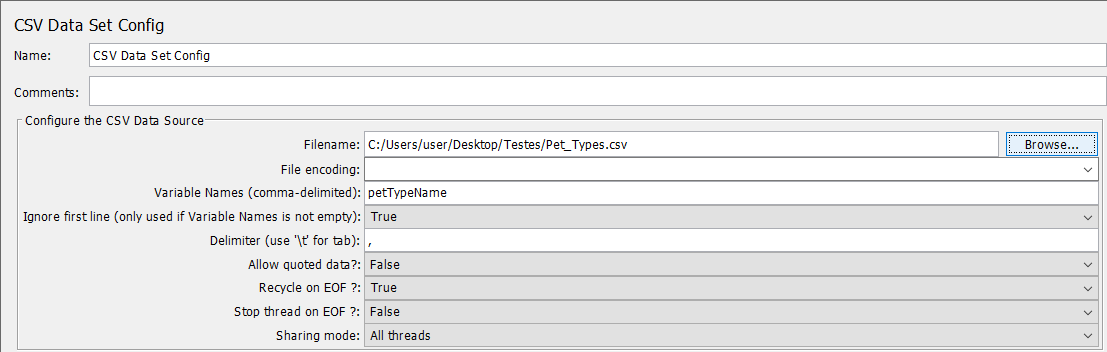
\includegraphics[width=\textwidth]{figs/Performance/jmeter/loadcsvJmeter.png}
	\caption{Load Data from CSV on jmeter}
	\label{fig:LoadCSVjmeter}
\end{figure}

\begin{figure}[H]
	\centering
	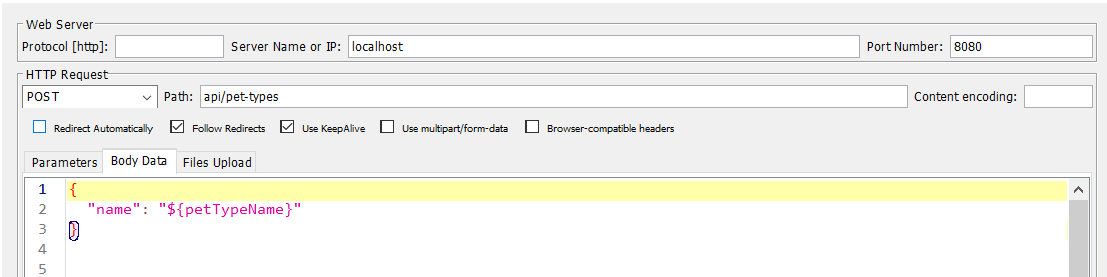
\includegraphics[width=\textwidth]{figs/Performance/jmeter/loadcsv2Jmeter.png}
	\caption{Use Data from CSV on jmeter}
	\label{fig:LoadCSV2jmeter}
\end{figure}

\begin{figure}[H]
	\centering
	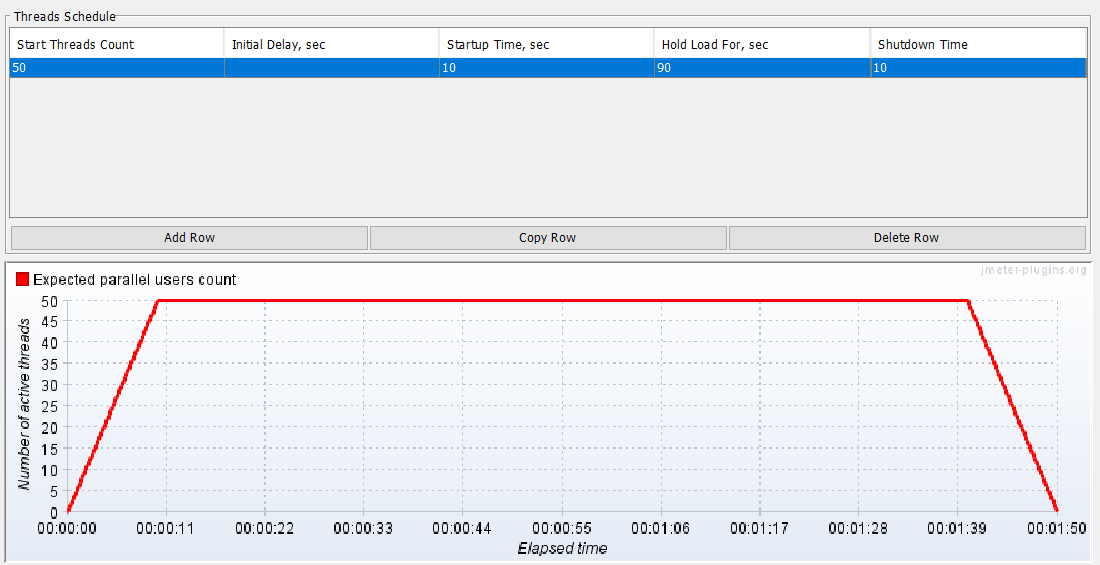
\includegraphics[width=\textwidth]{figs/Performance/jmeter/LoadJmeterConfiguration.png}
	\caption{Load Test Configuration on jMeter}
	\label{fig:LoadConfigurationjMeter}
\end{figure}

\begin{figure}[H]
	\centering
	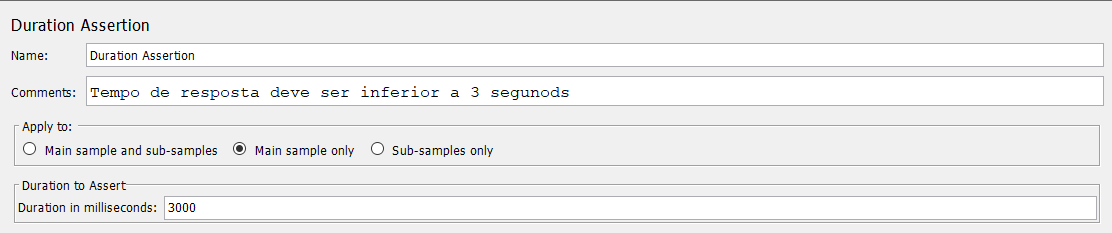
\includegraphics[width=\textwidth]{figs/Performance/jmeter/Load-SoakJmeterDurationAssertion.png}
	\caption{Load Duration Configuration on jMeter}
	\label{fig:LoadDurationjMeter}
\end{figure}




\textbf{Results}

In the figure \ref{fig:LoadAggregatejMeter} we can see the Aggregate Report of the jmeter test. In the figure \ref{fig:LoadResponsejMeter} we can see the response time over time of the jmeter test. 

\begin{figure}[H]
	\centering
	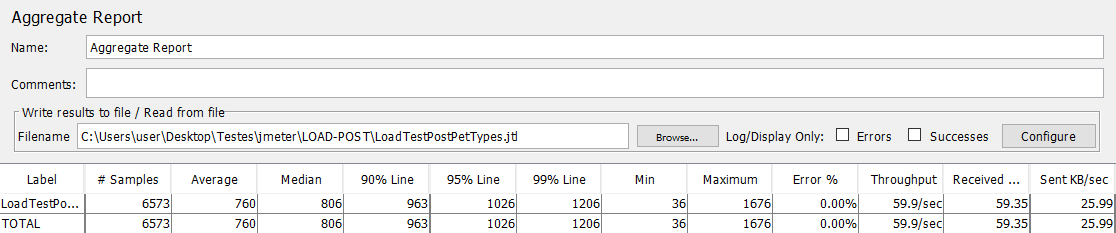
\includegraphics[width=\textwidth]{figs/Performance/jmeter/LoadPostAgregateResult.png}
	\caption{Load Aggregate Report}
	\label{fig:LoadAggregatejMeter}
\end{figure}

\begin{figure}[H]
	\centering
	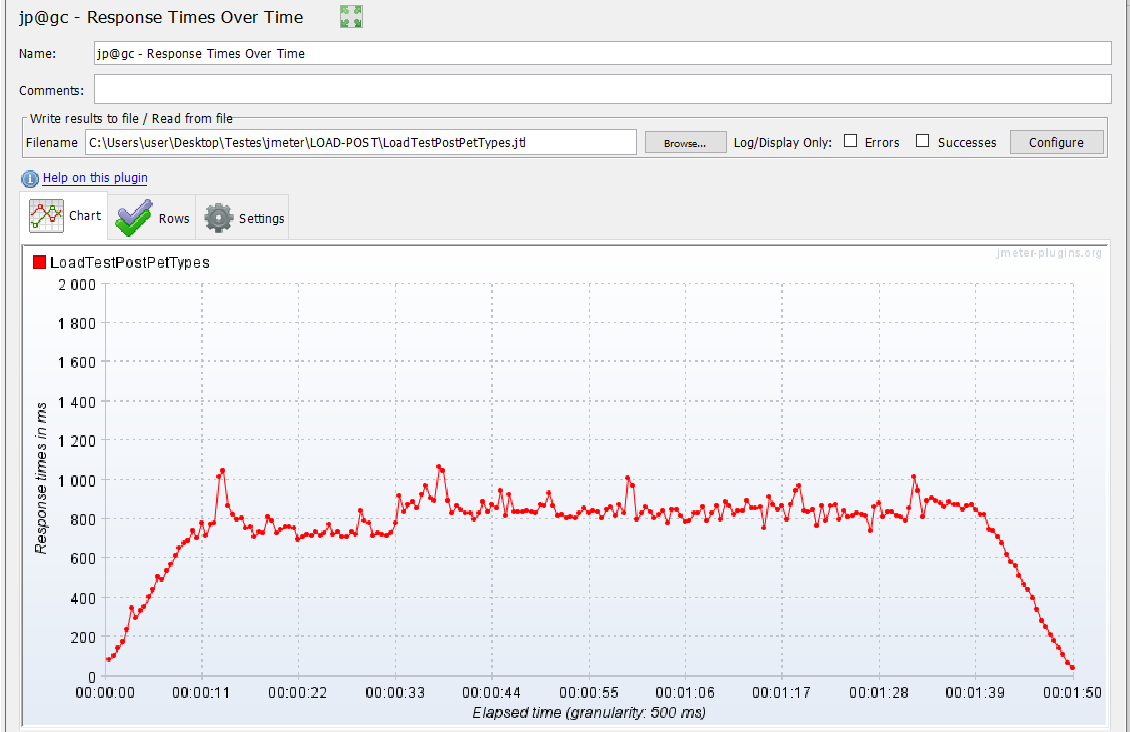
\includegraphics[width=\textwidth]{figs/Performance/jmeter/LoadPostResponsesOverTime.png}
	\caption{Load Response Time}
	\label{fig:LoadResponsejMeter}
\end{figure}

Based on these results, we can conclude that the application demonstrated solid performance throughout the load test. The maximum response time was recorded at 1.6 seconds, with no errors observed during the test. The response time graph indicates that the application maintained consistent performance over the test duration, with no significant deviations or performance degradation. Additionally, other key metrics, such as average response time and throughput, confirm the stability and reliability of the application under load.


\textbf{K6}




\textbf{Test Configuration}

In the figure \ref{fig:LoadCSVK6} we can see the configuration needed to load the csv file on K6, later, on the figure \ref{fig:LoadCSV2K6} we can see how to use the same data from the csv for the POST requests. In the figure \ref{fig:LoadConfigurationK6} we can see the configuration of the test for K6, where we can see that this test simulates a ramp-up to 50 virtual users over 10 seconds, maintains this load for 90 seconds, and then ramps down to 0 users over 10 seconds. Additionally, a performance threshold is defined to ensure that 99\% of HTTP request durations are below 3 seconds.


\begin{figure}[H]
	\centering
	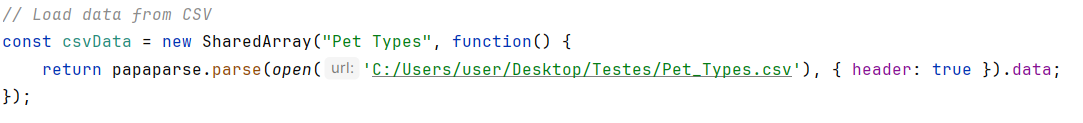
\includegraphics[width=\textwidth]{figs/Performance/k6/loadcsv1.png}
	\caption{Load Data from CSV on K6}
	\label{fig:LoadCSVK6}
\end{figure}

\begin{figure}[H]
	\centering
	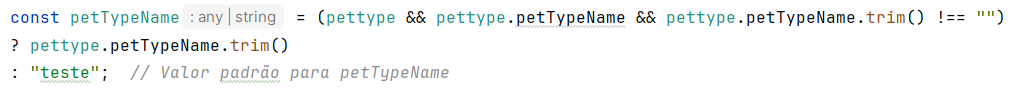
\includegraphics[width=\textwidth]{figs/Performance/k6/loadcsv2.png}
	\caption{Use Data from CSV on K6}
	\label{fig:LoadCSV2K6}
\end{figure}


\begin{figure}[H]
	\centering
	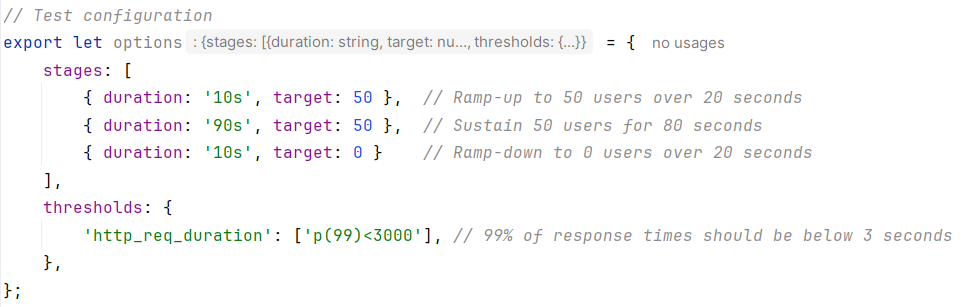
\includegraphics[width=\textwidth]{figs/Performance/k6/LoadPostK6.png}
	\caption{Load Configuration on K6}
	\label{fig:LoadConfigurationK6}
\end{figure}






\textbf{Results}

In the figure \ref{fig:LoadResultsK6} we can see the results of the k6 tests

\begin{figure}[H]
	\centering
	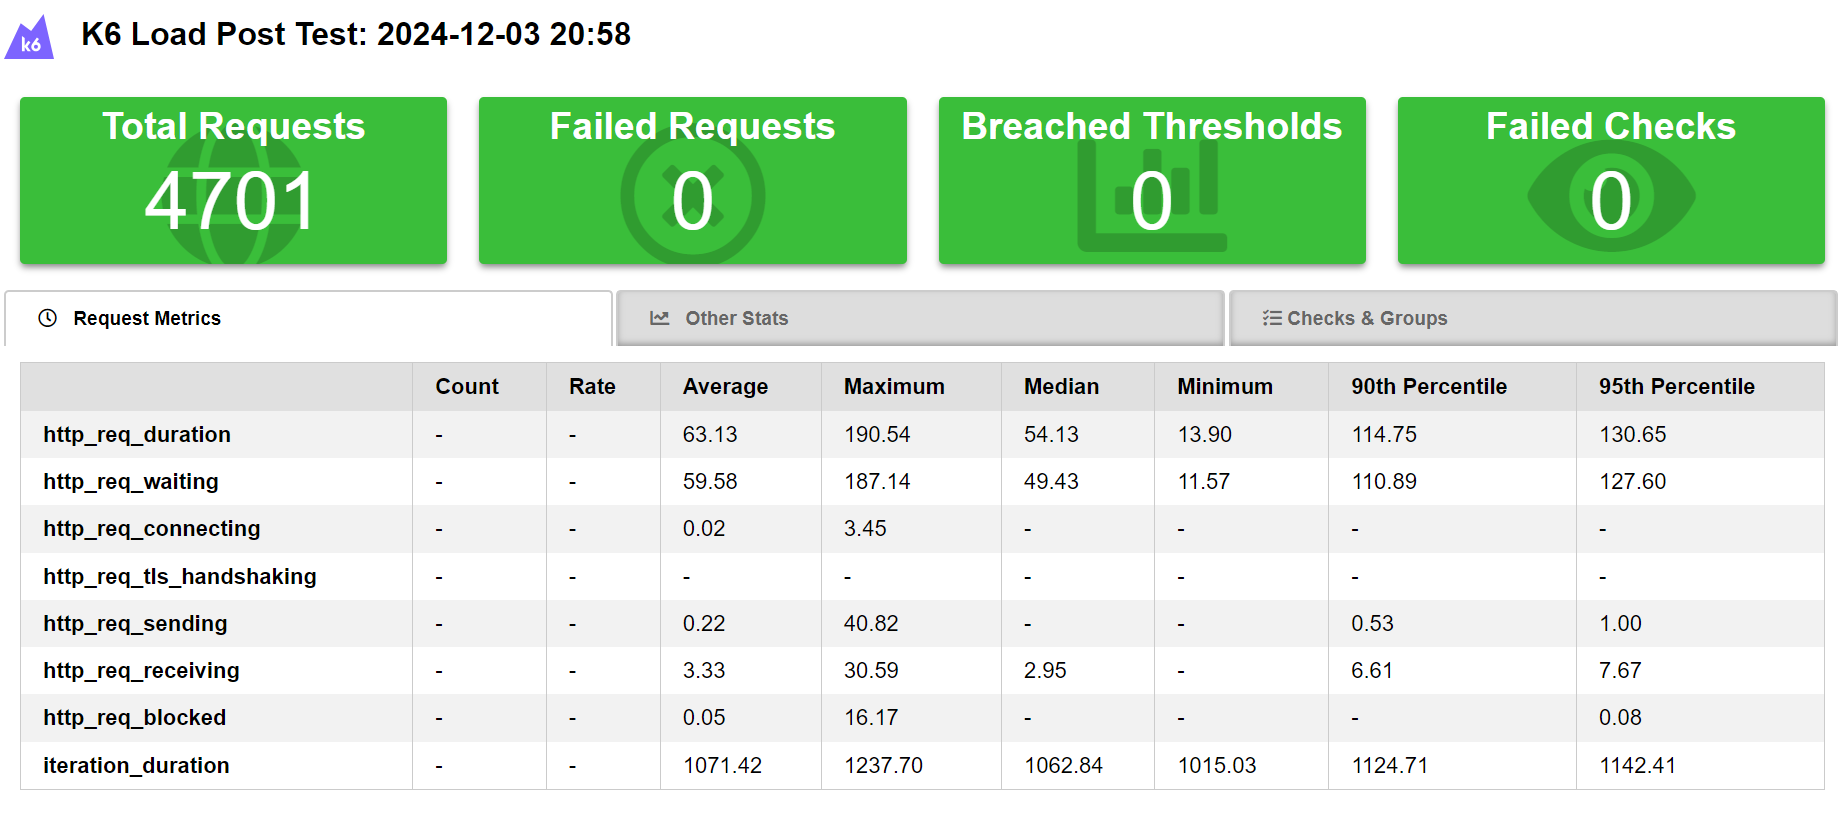
\includegraphics[width=\textwidth]{figs/Performance/k6/LoadPostK6Result.png}
	\caption{Load Results K6}
	\label{fig:LoadResultsK6}
\end{figure}

Based on these results, we can confidently state that the application performed with exceptional efficiency, handling a total of 4,701 requests with no errors, failed requests, or breached thresholds. The average response time was an impressive 61.15 milliseconds, and even at the 95th percentile, the response time remained under 121 milliseconds. The maximum response time recorded was just 130.56 milliseconds, showcasing the application's ability to maintain consistently low latency throughout the test.

\subsection{Soak Test}


Soak testing involves running a system at normal load levels for an extended period to identify performance issues that may not be apparent during shorter testing phases. This type of testing helps uncover problems such as memory leaks, resource depletion, and degradation in response times over time. By maintaining a steady load, soak tests provide insights into the system’s long-term reliability and stability, ensuring it can handle sustained usage without performance deterioration. In this section, we will evaluate the soak tests for the endpoint GET of petType.		
		
\textbf{Scenario GET}
\begin{itemize}
	\item 50 users of the web application
	\item Requesting all PetTypes
	\item The system returns a list with all PetTypes
	\item Normal Conditions
\end{itemize}


\textbf{Jmeter}





\textbf{Test Configuration}



In the figure \ref{fig:SoakConfigurationjMeter} we can see the configuration on jmeter for the test where we can see that the test simulates a ramp-up to 50 virtual users over 10 seconds, maintains this load for 700 seconds, and then ramps down to 0 users over 10 seconds. In the figure \ref{fig:SoakDurationjMeter} we can see the configuration for the duration for each request in jmeter of 3 seconds.



\begin{figure}[H]
	\centering
	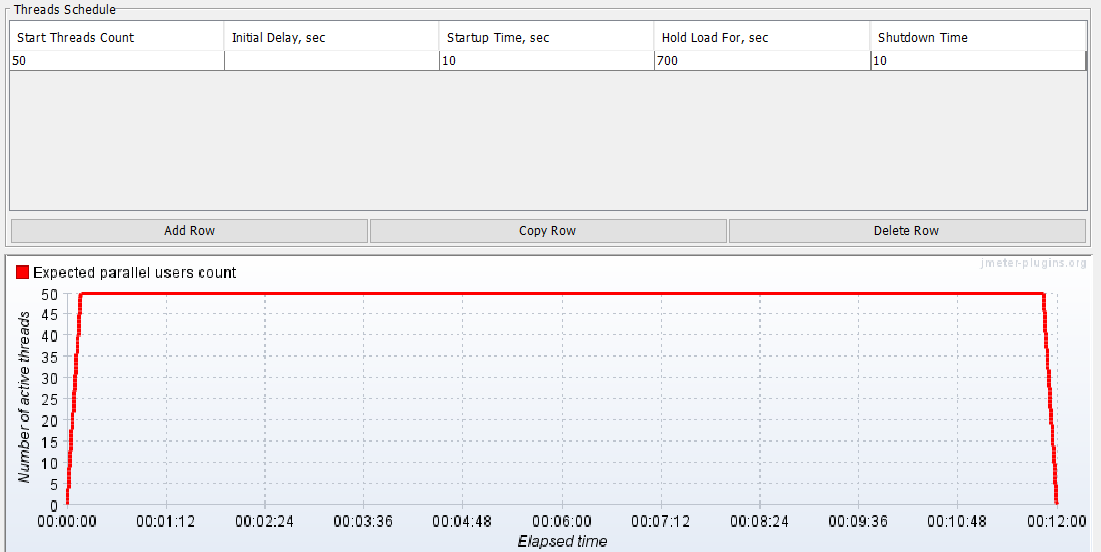
\includegraphics[width=\textwidth]{figs/Performance/jmeter/SoakJmeterConfiguration.png}
	\caption{Soak Test Configuration on jMeter}
	\label{fig:SoakConfigurationjMeter}
\end{figure}

\begin{figure}[H]
	\centering
	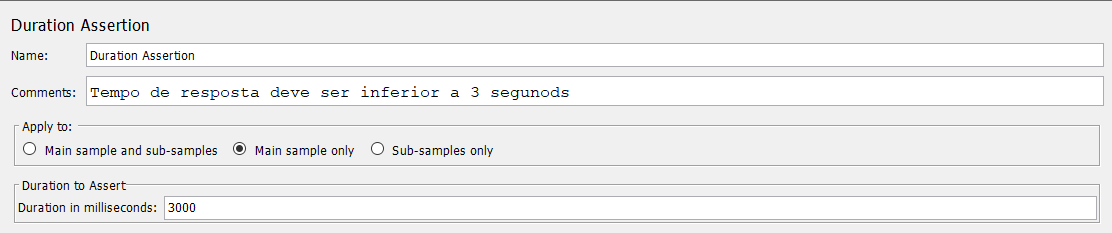
\includegraphics[width=\textwidth]{figs/Performance/jmeter/Load-SoakJmeterDurationAssertion.png}
	\caption{Soak Duration Configuration on jMeter}
	\label{fig:SoakDurationjMeter}
\end{figure}




\textbf{Results}

In the figure \ref{fig:SoakAggregatejMeter} we can see the Aggregate Report of the jmeter test. In the figure \ref{fig:SoakResponsejMeter} we can see the response time over time of the jmeter test.

\begin{figure}[H]
	\centering
	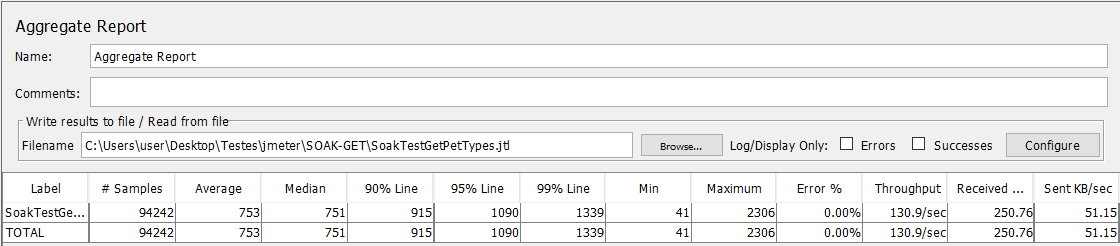
\includegraphics[width=\textwidth]{figs/Performance/jmeter/SoakGetAgregateResult.png}
	\caption{Soak Aggregate Report}
	\label{fig:SoakAggregatejMeter}
\end{figure}

\begin{figure}[H]
	\centering
	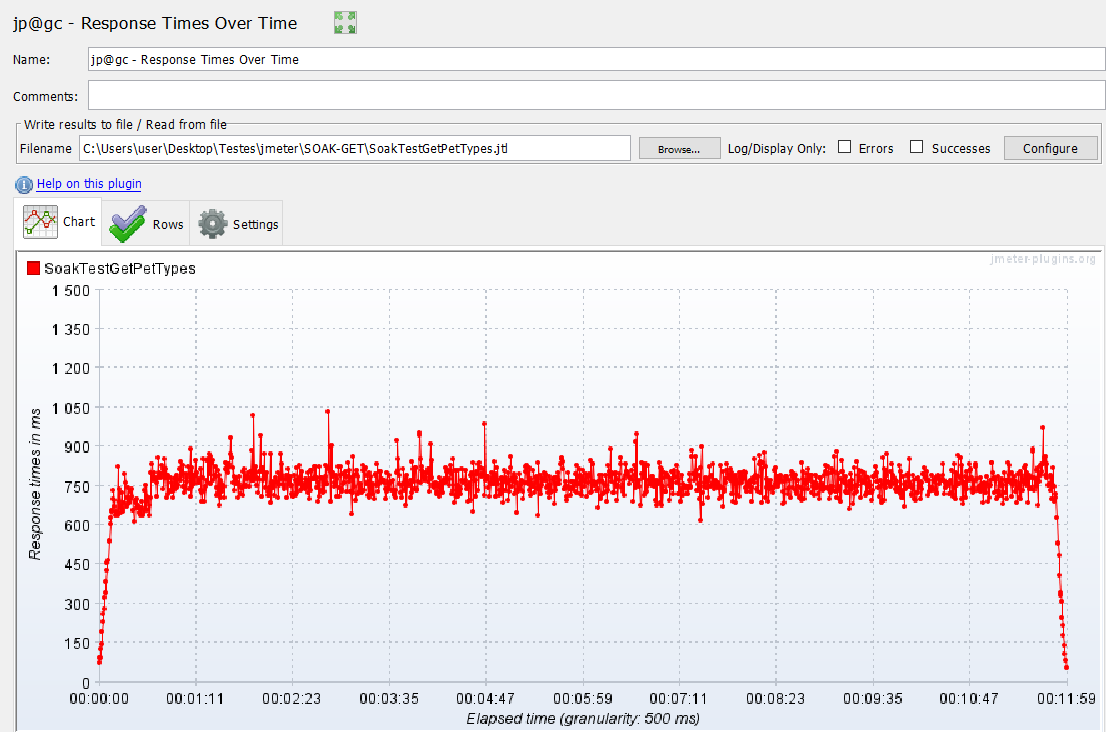
\includegraphics[width=\textwidth]{figs/Performance/jmeter/SoakGetResponsesOverTime.png}
	\caption{Soak Response Time}
	\label{fig:SoakResponsejMeter}
\end{figure}

From the results of the soak test, we can confirm that the application maintained stable performance over an extended period. A total of 94242 samples were processed, with a maximum response time of 2,306 second. The average response time was 753 milliseconds, indicating reliable performance under continuous load.

The response time graph shows steady behavior, with minor fluctuations that remained within an acceptable range throughout the test duration. This stability demonstrates the application's ability to handle sustained traffic without any signs of performance degradation.

\textbf{K6}



\textbf{Test Configuration}

In the figure \ref{fig:SoakConfigurationK6} we can see the configuration of the test for K6, where we can see that the test simulates a ramp-up to 50 virtual users over 10 seconds, maintains this load for 700 seconds, and then ramps down to 0 users over 10 seconds. Additionally, a performance threshold is set to ensure that 99\% of HTTP request durations are below 3 seconds


\begin{figure}[H]
	\centering
	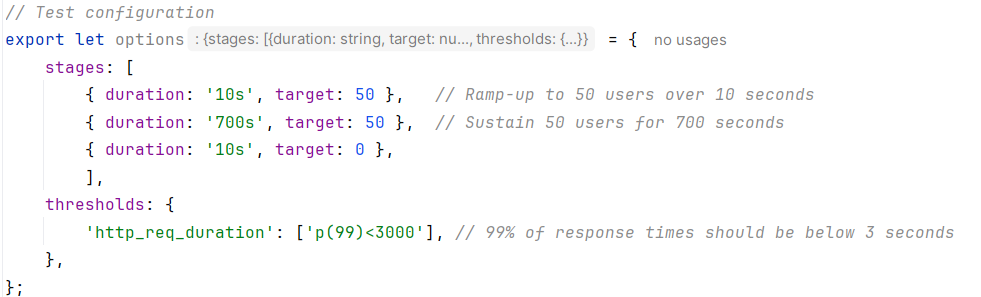
\includegraphics[width=\textwidth]{figs/Performance/k6/SoakGetK6.png}
	\caption{Soak Configuration on K6}
	\label{fig:SoakConfigurationK6}
\end{figure}






\textbf{Results}

In the figure \ref{fig:SoakResultsK6} we can see the results of the k6 test.

\begin{figure}[H]
	\centering
	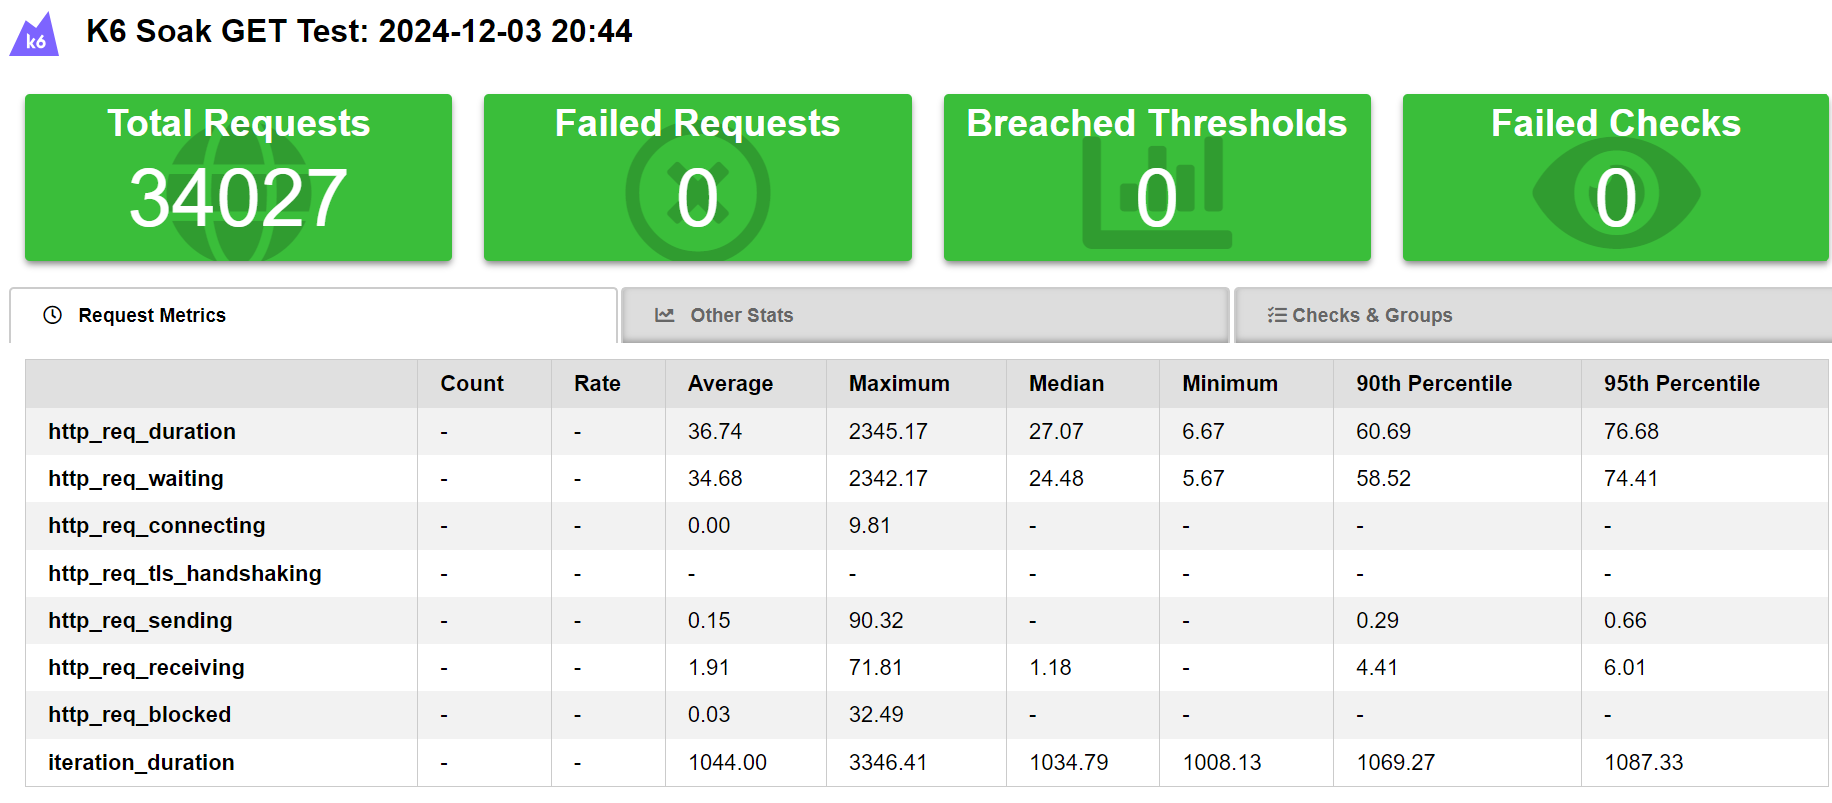
\includegraphics[width=\textwidth]{figs/Performance/k6/SoakGetK6Result.png}
	\caption{Soak Results K6}
	\label{fig:SoakResultsK6}
\end{figure}

Based on the results of the test, the application demonstrated excellent performance and stability, successfully handling a total of 34,027 requests with zero failed requests, breached thresholds, or failed checks. This indicates that the application was able to process all incoming traffic efficiently without any errors or performance issues.

The iteration duration metrics further highlight the application's consistency, with a median response time of 1,034 milliseconds and a maximum of 3,346 milliseconds. These results show that while the majority of requests were handled quickly, even the longest processing times remained within acceptable limits.

\subsection{Stress Test}
		
Stress testing is designed to push a system beyond its normal operational capacity to evaluate its robustness and determine its breaking point. Unlike soak testing, which focuses on long-term stability under sustained load, stress testing subjects the system to extreme load levels, such as a high volume of requests or rapid increases in traffic, to identify vulnerabilities and performance bottlenecks under peak conditions. This type of testing helps uncover issues such as response delays, crashes, or failures in handling surges. In this section, I will conduct a stress test for the endpoint GET of petType
\textbf{Scenario GET}
\begin{itemize}
	\item 200 users of the web application
	\item Requesting all PetTypes
	\item The system returns a list with all PetTypes
	\item Heavy Conditions
\end{itemize}


\textbf{Jmeter}



\textbf{Test Configuration}



In the figure \ref{fig:StressConfigurationjMeter} we can see the configuration on jmeter for the test where we can see that the test simulates a ramp-up to 200 virtual users over 10 seconds, sustains 200 users for 90 seconds, and then ramps down to 0 users over 10 seconds. In the figure \ref{fig:StressDurationjMeter} we can see the configuration for the duration for each request in jmeter of 5 seconds.



\begin{figure}[H]
	\centering
	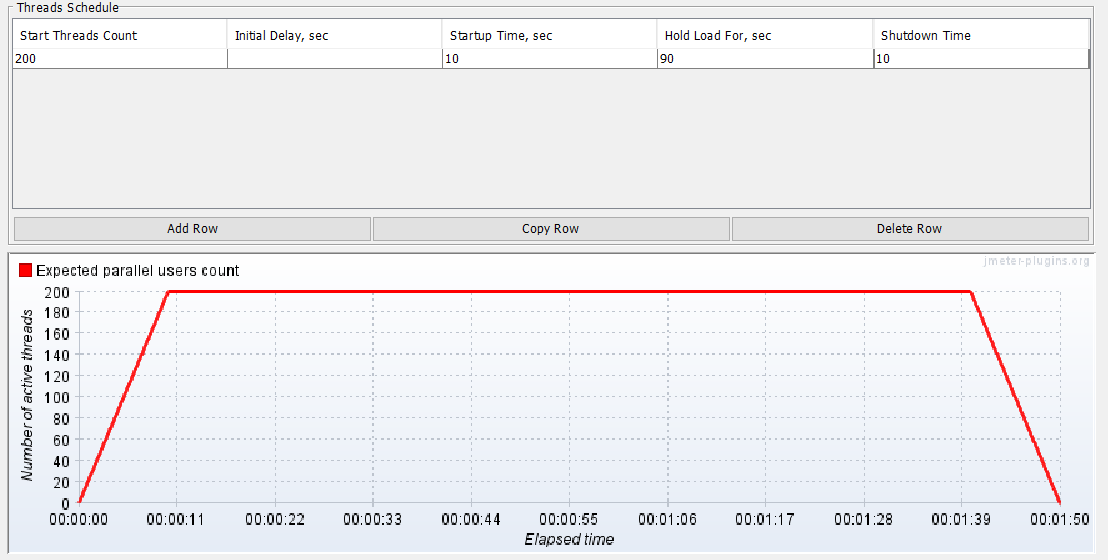
\includegraphics[width=\textwidth]{figs/Performance/jmeter/StressJmeterConfiguration.png}
	\caption{Stress Test Configuration on jMeter}
	\label{fig:StressConfigurationjMeter}
\end{figure}

\begin{figure}[H]
	\centering
	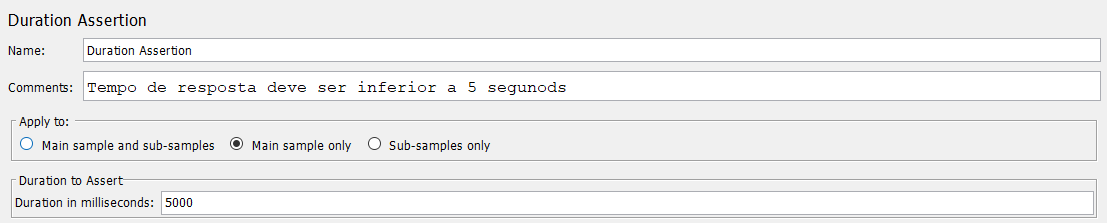
\includegraphics[width=\textwidth]{figs/Performance/jmeter/StressJmeterDurationAssertion.png}
	\caption{Stress Duration Configuration on jMeter}
	\label{fig:StressDurationjMeter}
\end{figure}




\textbf{Results}

In the figure \ref{fig:StressAggregatejMeter} we can see the Aggregate Report of the jmeter test. In the figure \ref{fig:SoakResponsejMeter} we can see the response time over time of the jmeter test.

\begin{figure}[H]
	\centering
	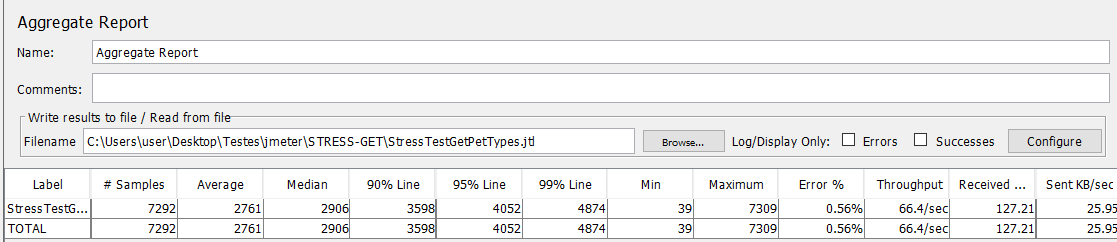
\includegraphics[width=\textwidth]{figs/Performance/jmeter/StressGetAgregateResult.png}
	\caption{Stress Aggregate Report}
	\label{fig:StressAggregatejMeter}
\end{figure}

\begin{figure}[H]
	\centering
	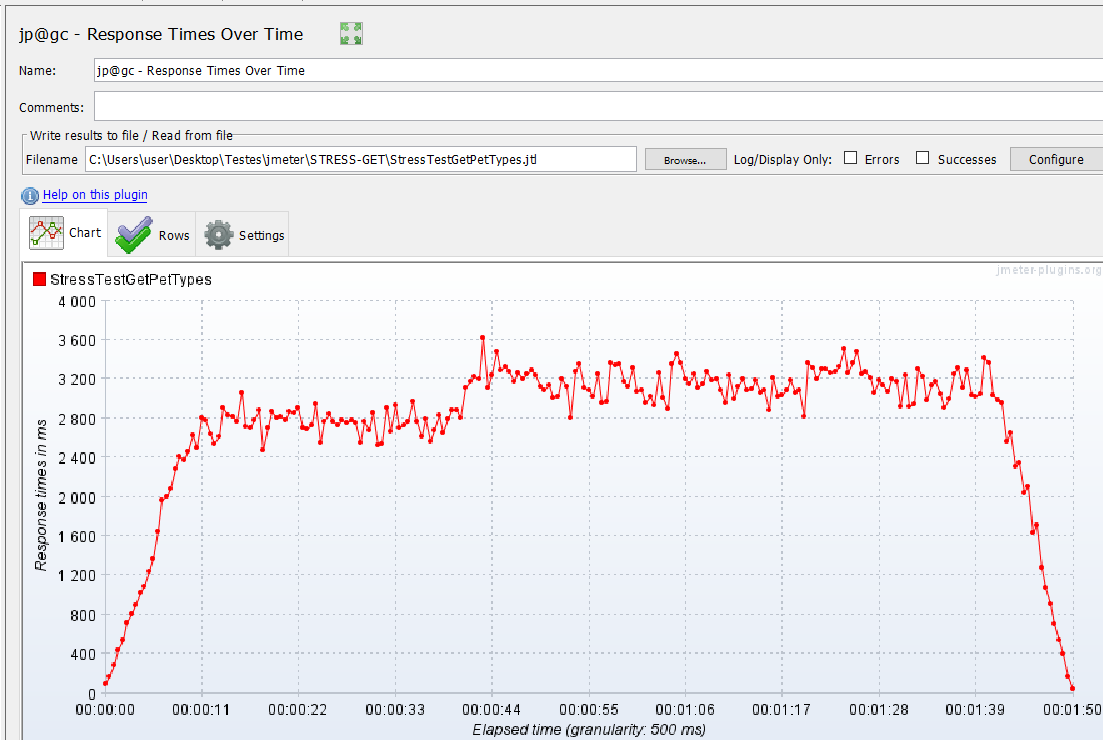
\includegraphics[width=\textwidth]{figs/Performance/jmeter/StressGetResponsesOverTime.png}
	\caption{Stress Response Time}
	\label{fig:StressResponsejMeter}
\end{figure}
 
From the results of the stress test, we can confirm that the application maintained stable performance with a heavy load. A total of 7292 samples were processed, with a maximum response time of 7,3 seconds. The average response time was 2761 milliseconds, indicating reliable performance under heavy load.

The response time graph shows steady behavior, with a minor fluctuations around 44 seconds, but remained within an acceptable range throughout the test duration. This stability demonstrates the application's ability to handle sustained traffic without any signs of performance degradation.


\textbf{K6}




\textbf{Test Configuration}



In the figure \ref{fig:StressConfigurationK6} we can see the configuration of the test for K6, where we can see that the test simulates a ramp-up to 200 virtual users over 10 seconds, sustains 200 users for 90 seconds, and then ramps down to 0 users over 10 seconds. Additionally, a performance threshold is defined to ensure that 95\% of HTTP request durations are below 5 seconds.



\begin{figure}[H]
	\centering
	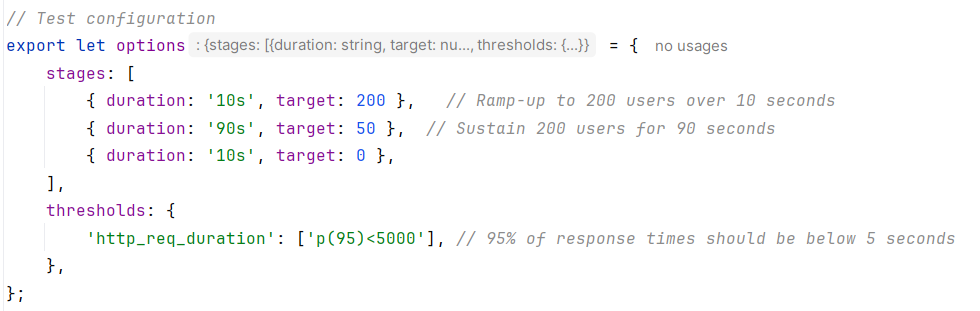
\includegraphics[width=\textwidth]{figs/Performance/k6/StressGetK6.png}
	\caption{Stress Configuration on K6}
	\label{fig:StressConfigurationK6}
\end{figure}




\textbf{Results}

In the figure \ref{fig:StressResultsK6} we can see the results of the k6 test.

\begin{figure}[H]
	\centering
	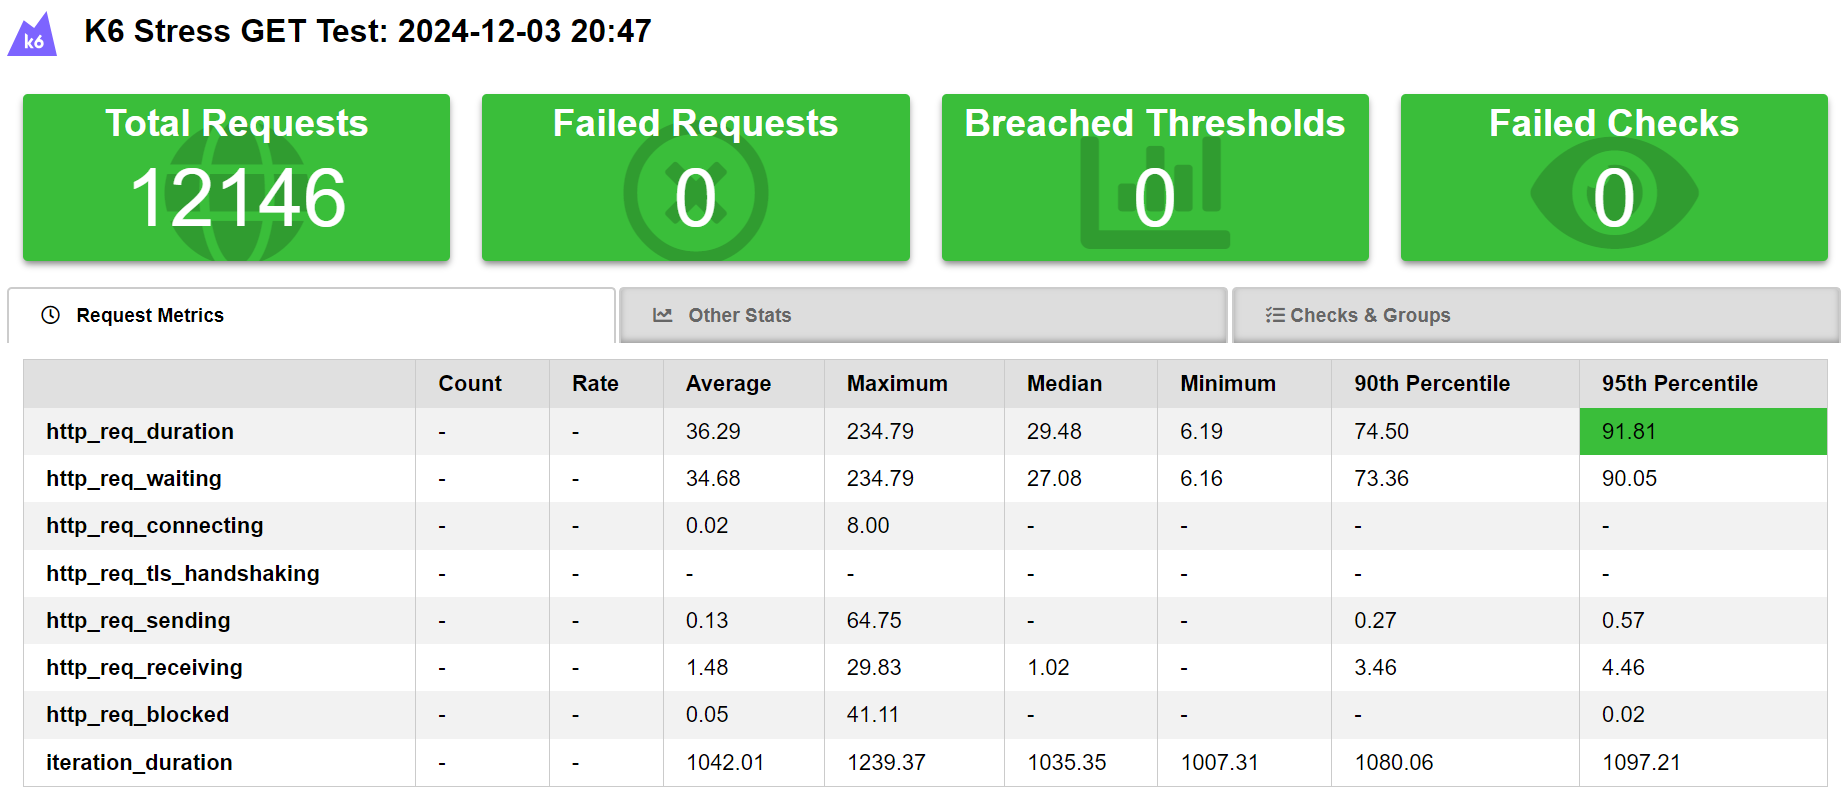
\includegraphics[width=\textwidth]{figs/Performance/k6/StressGetK6Result.png}
	\caption{Stress Results K6}
	\label{fig:StressResultsK6}
\end{figure}

Based on the results of the test, the application demonstrated excellent performance and stability, successfully handling a total of 12,146 requests with zero failed requests, breached thresholds, or failed checks. This indicates that the application was able to process all incoming traffic efficiently without any errors or performance issues.

The iteration duration metrics further highlight the application's consistency, with a median response time of 1,042 milliseconds and a maximum of 1,239 milliseconds. These results show that the requests were handled quickly, even the longest processing times remained within acceptable limits.



\section{Frontend Performance}
In this chapter, I focus on evaluating the frontend performance of the application, adopting a user-centric approach to ensure an optimal experience. Guided by the RAIL model Response, Animation, Idle, and Load—and aligned with Core Web Vitals, the analysis aims to highlight key metrics that impact user experience. By examining these aspects, I aim to identify strengths and areas for improvement, ensuring the frontend is well-suited to meet modern performance standards.
\subsection{LightHouse Report}
The frontend performance received an overall score of 59/100, as seen in the figure \ref{fig:LightHousePerformance} indicating room for improvement in achieving a smoother and faster user experience. 

\begin{figure}[H]
	\centering
	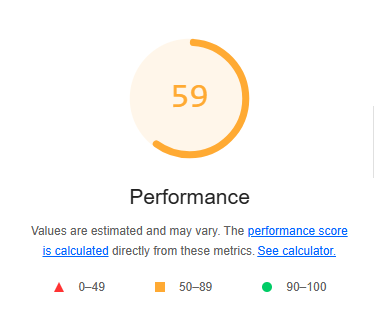
\includegraphics[width=.7\textwidth]{figs/Performance/Frontend/Lighthouse Performance.png}
	\caption{LightHouse performance Report}
	\label{fig:LightHousePerformance}
\end{figure}

In the figure \ref{fig:LighthouseMetrics} we have a breakdown of each metric evaluate, and on the figure \ref{fig:LighthouseImpact} we have the impact of each of those metrics for the final result.
\begin{figure}[H]
	\centering
	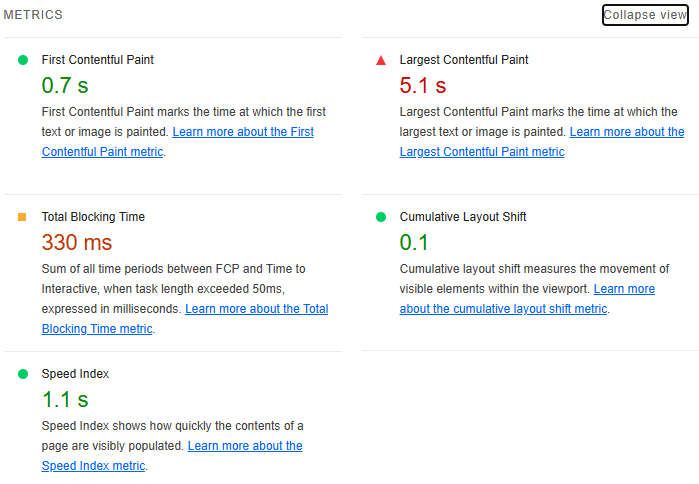
\includegraphics[width=.7\textwidth]{figs/Performance/Frontend/Lighthouse Metrics.png}
	\caption{Lighthouse Metrics Report}
	\label{fig:LighthouseMetrics}
\end{figure}

\begin{figure}[H]
	\centering
	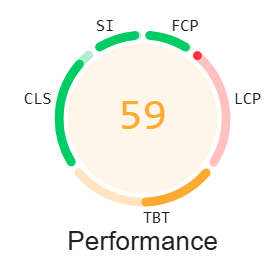
\includegraphics[width=.7\textwidth]{figs/Performance/Frontend/LighthouseImpact.png}
	\caption{Lighthouse Impact Report}
	\label{fig:LighthouseImpact}
\end{figure}


Below is a breakdown of the key metrics evaluated by Lighthouse:
\begin{itemize}
    \item \textbf{First Contentful Paint (FCP):} At 0.7 seconds (green), this metric is excellent, as it measures the time it takes for the first piece of content to appear on the screen. A fast FCP helps create a good initial impression for users.

    \item \textbf{Largest Contentful Paint (LCP):} At 5.1 seconds (red), this metric is too slow, measuring the time to render the largest visible element. It directly impacts how quickly users feel the page is fully loaded, and optimization is needed.

    \item \textbf{Total Blocking Time (TBT):} At 330 milliseconds (yellow), this metric measures delays caused by tasks that block interactivity. While acceptable, it can be improved by reducing JavaScript execution or deferring non-critical scripts.

    \item \textbf{Cumulative Layout Shift (CLS):} At 0.1 (green), this measures layout stability, ensuring that content doesn’t unexpectedly shift during loading. This result is excellent.

    \item \textbf{Speed Index:} At 1.1 seconds (green), this measures how quickly visible content is rendered. The score is outstanding, indicating fast rendering and a smooth visual experience.
\end{itemize}

By analyzing the diagnostics, on the figure \ref{fig:LCP} I found that one of the reasons for such poor LCP, was due to the Development Flag. This was also an issue on the accessibility. Removing this flag would most likely improve the Frontend Performance.

\begin{figure}[H]
	\centering
	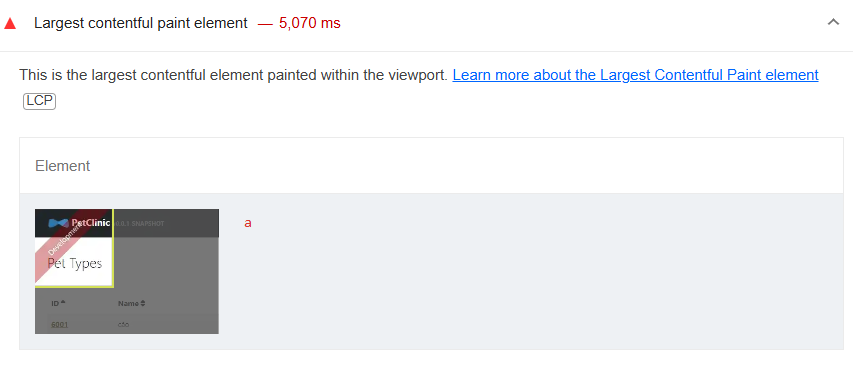
\includegraphics[width=.7\textwidth]{figs/Performance/Frontend/LCP Problem.png}
	\caption{LCP Element causing the problem}
	\label{fig:LCP}
\end{figure}


By removing the banner the results had a significant improvement. The application score a 69 out of 100.
\begin{figure}[H]
	\centering
	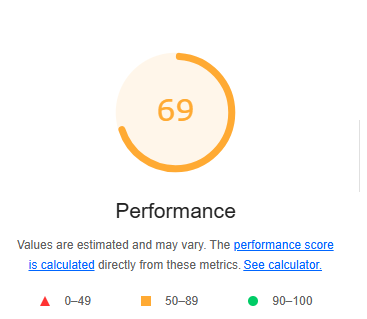
\includegraphics[width=.7\textwidth]{figs/Performance/Frontend/Lighthouse Performance after changes.png}
	\caption{LightHouse performance Report after changes}
	\label{fig:LightHousePerformanceAC}
\end{figure}

In the figure \ref{fig:LighthouseMetricsAC} we have a breakdown of each metric evaluate, and on the figure \ref{fig:LighthouseImpactAC} we have the impact of each of those metrics for the final result.
\begin{figure}[H]
	\centering
	\includegraphics[width=.7\textwidth]{figs/Performance/Frontend/Lighthouse Metrics after changes.png}
	\caption{Lighthouse Metrics Report after changes}
	\label{fig:LighthouseMetricsAC}
\end{figure}

\begin{figure}[H]
	\centering
	\includegraphics[width=.7\textwidth]{figs/Performance/Frontend/LighthouseImpact after changes.png}
	\caption{Lighthouse Impact Report after changes}
	\label{fig:LighthouseImpactAC}
\end{figure}

Although the changes were primarily intended to improve the LCP, the results showed a different outcome. Three metrics (TBT, CLS, and Speed Index) performed better; however, the metric we aimed to improve remained unchanged.

So, even though the result was not the intended one, I observed improvements in other areas, which suggests that the changes made had a positive overall impact.

\section{Conclusion}
In conclusion, the performance analysis revealed a mixed outcome. The frontend performance, as measured by Lighthouse, scored 59/100, reflecting significant issues with page responsiveness and loading times, particularly due to a poor Largest Contentful Paint (LCP) and Total Blocking Time (TBT). These metrics indicate the need for substantial optimization to improve the user experience.


The backend performance, however, demonstrated strong stability and reliability in most tests. Across various scenarios—load, stress, and soak tests—the system consistently processed requests without errors or failed checks.


Overall, while the backend shows promise, with reliable request handling and strong stability under heavy loads, response times could be further optimized. The frontend, on the other hand, requires considerable attention to meet modern performance standards. However, after the changes we saw the performance have a boost in its ratings. Combining both aspects, the performance for this iteration is rated 4 out of 5, acknowledging the solid backend performance but noting significant areas for improvement in the frontend.

%% =================================
	\chapter{Security}
\textit{	[Description, for what under individual responsibility, that inform the goal, the questions related to security, metrics used and their values, with partial response to questions, and goal achievement analysis. Explicitly mention the tool report(s).]}
		


	%% =================================
	\chapter{Conclusions }
	The individual report centered on analyzing a JHipster-generated application, focusing on key aspects such as accessibility, visual compatibility, maintainability, and performance. Both the frontend and backend were thoroughly tested using various tools, with each test and its methodology detailed in the respective chapters.

Through analysis and adjustments, it can confidently be stated that the application is in a solid state. There are several positive aspects highlighted across the tested topics, both of the frontend and backend, demonstrating its potential as a reliable foundation. While some areas require improvement, these shortcomings do not overshadow the overall quality and readiness of the application. It serves as a strong starting point for future development and enhancement, providing a robust base upon which more complex features and refinements can be built.
 ...\newline



	
	\bibliographystyle{ACM-Reference-Format}
	\renewcommand\bibname{References}
	\bibliography{ref}
	\label{references}
	\addcontentsline{toc}{chapter}{References}
	
\end{document}